\documentclass[12pt,a4paper]{article}

% Paquetes básicos
\usepackage[x11names]{xcolor}
\usepackage[utf8]{inputenc}
\usepackage{mathtools, amssymb, amsthm}
\usepackage{changepage}
\usepackage{geometry}
\usepackage[colorlinks=true]{hyperref}
\usepackage{enumitem}
\usepackage{etoolbox}
\usepackage{graphicx}
\usepackage{setspace}
\usepackage{tcolorbox}
\tcbuselibrary{skins, breakable}
\usepackage{titlesec}
\usepackage{tikz} % core TikZ
\usetikzlibrary{matrix}

% Margins
%\geometry{left=3cm,right=3cm,top=2.5cm,bottom=2.5cm}

% Custom operators
\newcommand{\card}{\operatorname{card}}

% Implication box setup
\tcbset{Implication-number/.style={
  enhanced,
  boxsep=2pt,
  colback=white,
  frame hidden,
  sharp corners,
  left=2pt, right=2pt, top=1pt, bottom=1pt,
  underlay={
    \draw[line width=0.5pt] (frame.south west) -- ([xshift=-133mm]frame.south east); % línea horizontal
    \draw[line width=0.5pt] ([xshift=-133mm]frame.north east) -- ([xshift=-133mm]frame.south east); % línea vertical
  }
}}

\tcbset{Implication-number-ds/.style={
  enhanced,
  boxsep=2pt,
  colback=white,
  frame hidden,
  sharp corners,
  left=2pt, right=2pt, top=1pt, bottom=1pt,
  underlay={
    \draw[line width=0.5pt] ([yshift=5mm]frame.south west) -- ([xshift=-133mm, yshift=5mm]frame.south east); % línea horizontal
    \draw[line width=0.5pt] ([xshift=-133mm, yshift=-3mm]frame.north east) -- ([xshift=-133mm, yshift=5mm]frame.south east); % línea vertical
  }
}}

\tcbset{Subset-contingency/.style={
  enhanced,
  boxsep=2pt,
  colback=white,
  frame hidden,
  sharp corners,
  left=2pt, right=2pt, top=1pt, bottom=1pt,
  underlay={
    \draw[line width=0.5pt] (frame.south west) -- ([xshift=-140mm]frame.south east); % línea horizontal
    \draw[line width=0.5pt] ([xshift=-140mm]frame.north east) -- ([xshift=-140mm]frame.south east); % línea vertical
  }
}}

\tcbset{Indent-subset-contingency/.style={
  enhanced,
  boxsep=2pt,
  colback=white,
  frame hidden,
  sharp corners,
  left=2pt, right=2pt, top=1pt, bottom=1pt,
  underlay={
    \draw[line width=0.5pt] (frame.south west) -- ([xshift=-140mm+0.07\textwidth]frame.south east); % línea horizontal
    \draw[line width=0.5pt] ([xshift=-140mm+0.07\textwidth]frame.north east) -- ([xshift=-140mm+0.07\textwidth]frame.south east); % línea vertical
  }
}}

% Useful commands
\renewcommand{\contentsname}{Contenidos}

\newcommand{\R}{\mathbb{R}}
\newcommand{\N}{\mathbb{N}}
\newcommand{\Z}{\mathbb{Z}}
\newcommand{\Q}{\mathbb{Q}}
\newcommand{\C}{\mathbb{C}}

\newcommand{\smallcup}{\mathop{\cup}\limits}
\newcommand{\smallcap}{\mathop{\cap}\limits}
\newcommand{\smallsum}{\mathop{\sum}\limits}
\newcommand{\smallprod}{\mathop{\prod}\limits}

\newcommand{\linf}[1]{\displaystyle{\mathop{\underline{\lim}}_{#1}}}
\newcommand{\mlim}[1]{\displaystyle{\lim_{#1}}}

%Integral de Lebesgue con patas
\newcommand{\lbint}{\mathop{\int_{\!\!\!\!\!|\!}^{\!|\!}}}

% ----- Custom counters and counter commands -----
% Custom counter hierarchy
\newcounter{unit}[section]
\newcounter{chapter}[unit]
\makeatletter
\@addtoreset{subsubsection}{chapter}
\makeatother

\renewcommand{\theunit}{\arabic{unit}}
\renewcommand{\thechapter}{\arabic{chapter}}
\renewcommand{\thesubsubsection}{\theunit.\thechapter.\arabic{subsubsection}}

% Custom content hierarchy behavior
\newcommand{\chapter}[1]{
    \refstepcounter{chapter}
    \subsection*{\Large{\S \thechapter. #1}}
    \addcontentsline{toc}{subsection}{\thechapter. #1}
}
\newcommand{\unit}[1]{
    \refstepcounter{unit}
    \section*{\Huge{\Roman{unit} #1}}
    \addcontentsline{toc}{section}{\Roman{unit} #1}
}

\newcommand{\result}[1]{%
  \subsubsection{#1}%
  \label{result:\thesubsubsection}
}
  
\titleformat{\subsubsection}
    {\normalfont\large\bfseries} % mismo tamaño que \subsection
    {\thesubsubsection}{1em}{}
  
%---- Custom proof commands-----
\newcommand{\dem}{
    \noindent \underline{\textbf{Demostración:}}
}
\newcommand{\nota}{
    \noindent \underline{\textbf{Nota:}}
}
% ----------------------------------------
\hbadness=10000
\vbadness=10000
\hfuzz=100pt
\vfuzz=100pt
%------------------------------
\title{Análisis Matemático III}
\author{Javier Ortín Rodenas}
\date{Curso 2025-2026}

\begin{document}

\maketitle
\newpage
\hypersetup{linkcolor=black}
\tableofcontents
\hypersetup{linkcolor=Ivory4}
\newpage
\setcounter{unit}{1}
\unit{Integral de Lebesgue}
\chapter{Integral de Lebesgue para funciones no negativas}
\result{Convenio \texorpdfstring{$0 \cdot \infty$}{0 · infty}}
\hspace{3mm} Consideramos $0 \cdot \infty = 0$ siempre y cuando al menos uno de los dos factores represente la medida de algún conjunto.

\hspace{4mm}
\result{Definición de integral de funciones simples}
\hspace{3mm} Dado un espacio de medida $(X, \Sigma, \mu)$ y una función simple medible
\begin{align*}
    s: X \longrightarrow [0, +\infty) && \text{ con expresión canónica } s = \sum_{i = 1}^n \lambda_i X_{A_i}
\end{align*}
Definimos la integral de Lebesgue de $s$ sobre $X$ como el número:
$$\lbint_X s \,d\mu = \sum_{i=1}^{n} \lambda_i \cdot \mu(A_i)$$

\nota Implícitamente, ya está definida la integral de $s$ sobre $\Sigma(E) \hspace{2mm } \forall \hspace{1mm} E \in \Sigma$:
$$\lbint_E s \,d \mu = \lbint_X s_{|E} \,d\mu = \sum_{i=1}^{n}\lambda_i \cdot \mu(E \cap A_i)$$

\newpage
\result{Linealidad del integrando}
\hspace{3mm} Dado un espacio de medida $(X, \Sigma, \mu)$. Sea $s: X \longrightarrow [0, \infty)$ una función simple y medible. Sean $\{E_i\}_{i\in\N}$ con $i \neq j \Rightarrow E_i \cap E_j = \varnothing$. Entonces, se cumple:
$$\lbint_{\smallcup_{i\in\N}E_i} s \, d\mu = \sum_{i=1}^\infty \lbint_{E_i}s\,d\mu$$

\vspace{3mm}
\dem Sea $s = \displaystyle \sum_{i=1}^{n} \lambda_i \cdot X_{A_i}$ la expresión canónica de $s$. Entonces,
\begin{flalign*}
    &\lbint_{\smallcup_{i\in\N}E_i}s\,d\mu = \sum_{i=1}^{n} \lambda_i \cdot \mu\big(A_i \cap \smallcup_{i\in\N}E_i\big) = \sum_{i=1}^n \lambda_i \sum_{j=1}^\infty \mu(A_i \cap E_j) = \\
    &= \sum_{i=1}^n \left(\sum_{j=1}^\infty \lambda_i \cdot \mu(A_i \cap E_j) \right) = \sum_{j=i}^\infty \sum_{i=1}^n \lambda_i \cdot \mu(A_i \cap E_j) = \sum_{j=1}^{\infty} \lbint_{E_j}s\,d\mu
\end{flalign*}

\vspace{6mm}
\result{Linealidad parcial}
\hspace{3mm} Sea $(X, \Sigma, \mu)$ un espacio de medida. Sean $s,t : X \longrightarrow [0, \infty)$ funciones simples y medibles. Entonces, se cumple:
$$\lbint_{X}s + t\,d\mu = \lbint_{X}s\,d\mu + \lbint_{X}t\,d\mu$$

\vspace{2mm} \dem Sean sus expresiones canónicas las siguientes:
\begin{align*}
    s = \sum_{i=1}^{n} \alpha_i \cdot \mu(A_i) && t = \sum_{j=1}^m \beta_j \cdot \mu(B_j)
\end{align*}
Entonces, como $\{A_i\}_{i=1}^n$ y $\{B_j\}_{j=1}^m$ son recubrimientos disjuntos de $X$, se tiene:
\begin{flalign*}
    \lbint_{X}s\,d\mu = \sum_{i=1}^n \alpha_i \sum_{j=1}^{m} \mu(A_i \cap B_j) = \sum_{\substack{1\leq i \leq n \\ 1 \leq j \leq m}} \alpha_i \cdot \mu(A_i \cap B_j) \\
    \lbint_{X}t\,d\mu = \sum_{j=1}^m \beta_j \sum_{i=1}^{n} \mu(A_i \cap B_j) = \sum_{\substack{1\leq i \leq n \\ 1 \leq j \leq m}} \beta_j \cdot \mu(A_i \cap B_j)
\end{flalign*}
Sumando ambas expresiones obtenemos:
\begin{flalign*}
    \lbint_{X}&s\,d\mu + \lbint_{X}t\,d\mu = \sum_{\substack{1\leq i \leq n \\ 1 \leq j \leq m}} (\alpha_i + \beta_j) \cdot \mu(A_i \cap B_j) = \\
    &= \sum_{\substack{1\leq i \leq n \\ 1 \leq j \leq m}} \lbint_{A_i \cap B_j}s + t\,d\mu = \lbint_{X}s+t\,d\mu
\end{flalign*}
La última igualdad se deduce de la \hyperref[result:2.1.3]{linealidad del integrando}.

\hspace{4mm}
\result{Monotonía de la integral simple}
\hspace{3mm} Sea $(X, \Sigma, \mu)$ un espacio de medida. Sean $s, t: X \longrightarrow [0, \infty)$ funciones medibles simples tales que $s(x) \leq t(x) \forall x \in X$. Entonces, se cumple:
$$\lbint_{X}s\,d\mu \leq \lbint_{X}t\,d\mu$$

\vspace{2mm} \dem Sean sus expresiones canónicas: $\displaystyle s= \sum_{i=1}^n \alpha_i \cdot X_{A_i} \hspace{3mm} t = \sum_{j=1}^m \beta_j \cdot X_{B_j}$.
\begin{align*}
    \lbint_{X}s\,d\mu = \sum_{\substack{1\leq i \leq n\\1\leq j \leq m}} \alpha_i \mu(A_i \cap B_j) &&
    \lbint_{X}t\,d\mu = \sum_{\substack{1\leq i \leq n\\1\leq j \leq m}} \beta_j \mu(A_i \cap B_j)
\end{align*}
\indent Por hipótesis, tenemos que $s(x) \leq t(x)$ para todo $x\in X$. De este modo; sean $i \in \{1,\ldots,n\}, j \in \{1,\ldots, m\}$ cualesquiera, tenemos que o bien $\alpha_i \leq \beta_j$ o bien $A_i \cap B_j = \varnothing \Rightarrow \mu(A_i \cap B_j) = 0$. Por tanto, cada sumando del sumatorio de la izquierda va a ser menor o igual que el término de mismos índices del sumatorio de la derecha, hemos demostrado el resultado.

\vspace{6mm}
\result{Linealidad de la integral simple por constantes}
\hspace{3mm} Sea $(X, \Sigma, \mu)$ un espacio de medida. Sea $\displaystyle s = \sum_{i=1}^n \lambda_i \cdot X_{A_i}$ una función simple, medible y no negativa. Entonces:
$$\lbint_{X}c \cdot s\,d\mu = c \cdot \lbint_{X}s\,d\mu \hspace{4mm} \forall c \in \R$$
\vspace{2mm} \dem Distinguimos dos casos:
\begin{itemize}
    \item Si $c = 0$, entonces $s \cdot c \equiv 0$ y se cumple:
    $$\lbint_{X}c \cdot s\,d\mu = \lbint_{X}0\,d\mu = 0 \cdot \mu(X) = 0 = 0 \cdot \lbint_{X}s\,d\mu$$
    \item Si $c \neq 0$, entonces:
    $$\lbint_{X}c\cdot s\,d\mu = \sum_{i=1}^{n} c \cdot \lambda_i \cdot X_{a_i} = c \cdot \sum_{i=1}^n \lambda_i \cdot \mu(X_{A_i}) = c \cdot \sum_{i=1}^n \lambda_i \cdot \mu(A_i) = c \cdot \lbint_{X}s\,d\mu $$
\end{itemize}

\vspace{6mm}
\result{Integral de funciones medibles no negativas}
\hspace{3mm} Sea $(X, \Sigma, \mu)$ un espacio de medida. Sea $f : X \longrightarrow [0, +\infty]$ medible. Se define la integral de Lebesgue de $f$ sobre $X$ como:
$$\int_{X}f\,d\mu = \sup\left\{\lbint_{X}s\,d\mu \hspace{2mm} \text{ con } 0 \leq s \leq s, \hspace{1mm} s \text{ función simple medible}\right\} = \sup \mathcal{S}_X(f)$$
Nótese que el conjunto anterior no es vacío, pues $s \equiv 0$ está en él. Además, se puede extender la definición anterior a cualquier subconjunto medible de $X$.

\vspace{6mm}
\result{Ejemplos de integrales}
\hspace{3mm} $\romannumeral 1)$ Función de Dirichlet: $X_\Q$. \newline Consideramos el espacio de medida $\big([0,1], \mathfrak{M}_1([0,1]), \mu_1\big)$. Esta función no es integrable en el sentido de Riemann, pues las sumas inferiores son siempre nulas y las superiores toman valor $1$ (se debe a la densidad de los racionales y los irracionales). Veamos que $X_\Q$ sí es integrable en el sentido de Lebesgue.
\newline \vspace{4mm} \indent Tenemos que $X_\Q$ es una función simple, pues toma el valor $1$ en $[0,1]\cap \Q$, que es numerable, y el valor $0$ en $[0,1]\setminus \Q$, que es medible al ser el complementario del conjunto anterior en este espacio de medida. Su integral viene dada por:
$$\lbint_{[0,1]}X_\Q\,d\mu = 1 \cdot \mu([0,1] \cap \Q) + 0 \cdot \mu([0,1] \setminus \Q) = 1 \cdot 0 + 0 \cdot 1 = 0$$
\vspace{4mm} \indent $\romannumeral 2)$ Consideramos el mismo espacio de medida que en el caso anterior. Veamos que la función de Thomae es integrable. Se define como sigue:
$$f(x) = \begin{cases}
    0 &\text{ si } x \in \Q\cap[0,1] \cup \{0\} \\
    \frac{1}{q} &\text{ si } x = \frac{p}{q} \text{ para }p,q \text{ naturales primos entre sí}
\end{cases} $$
\indent Sabemos por Análisis Matemático II que esta función es integrable-Riemann en $[0,1]$ con valor de su integral igual a $0$. Veamos que ocurre lo mismo con la integral de Lebesgue. Sea $s$ una función simple medible tal que $0 \leq s \leq f$. Se cumple $M := \max s([0,1]) \leq 1$. Los puntos donde $s$ toma valores positivos son a lo sumo numerables, pues se cumple:
$$f^{-1}\big((0, +\infty)\big) = \bigcup_{n\in\N} \bigcup_{i=1}^n \frac{i}{n}$$
Los puntos donde $s$ toma valores positivos han de estar contenidos en el conjunto anterior, que es numerable y tiene por tanto medida nula. De este modo, tenemos:
$$0 \leq \lbint_{[0,1]}s\,d\mu = 0 \mu\big(s^{-1}(\{0\})\big) + M \cdot \mu\Big(s^{-1}\big((0,M]\big)\Big) = 0$$

\vspace{6mm} \result{Propiedades básicas}
\hspace{3mm}  Sea $(X, \Sigma, \mu)$ un espacio de medida. Sean $f,g : X \leftarrow [0, \infty]$ funciones medibles. Sean $E,F \in \Sigma$. Sea $c \in [0, +\infty)$. Se cumplen los siguientes enunciados:
\begin{enumerate}[label=\roman*)]
    \item $0 \leq f \leq g \Rightarrow \int_{X}f\,d\mu \leq \int_{X}g\,d\mu$
    \item $\int_{X}c \dot f\,d\mu = c \cdot \int_{X}f\,d\mu$
    \item $f\equiv 0 \Rightarrow \int_{X}f\,d\mu = 0$
    \item $\mu(E) = 0 \leq \int_{E}f\,d\mu = 0$
    \item Si $E \subseteq F$; entonces, $\int_{E}f\,d\mu = \int_{D}f \cdot X_E\,d\mu$ y $\int_{E}f\,d\mu \leq \int_{D}f\,d\mu$
\end{enumerate}
\vspace{2mm} \dem \newline \vspace{2mm} $\romannumeral 1)$ Sea $s : X \longrightarrow [0, +\infty)$ una función simple medible tal que $s \leq f$. Entonces se cumple $s \leq g$. Por tanto, siguiendo la notación del \hyperref[result:2.1.7]{resultado 2.1.7}, tenemos que $\mathcal{S}_X(f) \subseteq \mathcal{S}_X(g)$ luego ha de cumplirse: $$\int_{X}f\,d\mu = \sup \mathcal{S}_X(f) \leq \sup \mathcal{S}_X(g) = \int_{X}g\,d\mu$$

\vspace{4mm} $\romannumeral 2)$ Distinguimos dos casos: En primer lugar, si $c = 0$ se tiene: $$\int_{X}c \cdot f\,d\mu = \int_{X}0\,d\mu = 0 = 0 \cdot \int_{X}f\,d\mu$$
Si $c \in (0, +\infty)$; entonces, tenemos:
\begin{flalign*}
    c \cdot \int_{X}f\,d\mu & = c \cdot \sup \left\{\lbint_{X}s\,d\mu : \hspace{2mm} 0 \leq s \leq f \hspace{2mm} \text{ con } s \text{ función medible simple}\right\} = \sup c \cdot \mathcal{S}_X(f)\\
    \int_{X}c\cdot f\,d\mu & \sup \left\{\lbint_{X}s\,d\mu : \hspace{2mm} 0 \leq t \leq c\cdot f \hspace{2mm} \text{ con } t \text{ función medible simple}\right\} = \sup \mathcal{S}_X(c\cdot f)
\end{flalign*}
Al cumplirse $c \in (0,+\infty)$, tenemos que $0 \leq f \leq s \iff 0 \leq c \cdot s \leq c \cdot f$ luego las integrales han de coincidir.

\vspace{6mm} $\romannumeral 3$  $\romannumeral 4)$ Trivial.

\vspace{4mm} $\romannumeral 5)$ Comencemos por ver la primera parte. Sea una función simple y medible $s : F \longrightarrow [0, +\infty)$ tal que $s \leq f \cdot X_E$. Entonces se tiene $s_{|E}$ es simple también. Además, se cumple:
$$\lbint_{F}s\,d\mu = \lbint_{E}s_{|E}\,d\mu + \lbint_{F \setminus E}0\,d\mu = \int_{E}s_{|E}\,d\mu$$
De manera similar, sea $t : E \longrightarrow [0,+\infty)$ simple tal que $t \leq f$, podemos extender $t$ a $F$ al considerar $\hat{t}(x) = t(x)$ si $x \in E$ ó $0$ si $x F \setminus E$. La función resultante $\hat{t}$ es simple, medible y cumple $\hat{t} \leq f \cdot X_E$. De este modo,
$$\lbint_{F}\hat{t}\,d\mu = \int_{F \setminus E}0\,d\mu + \lbint_{E}\hat{t}\,d\mu = \lbint_{E}t\,d\mu$$
Por tanto, se cumple $\mathcal{S}_E(f) = \mathcal{S}_F(f \cdot X_E)$ luego las integrales coinciden.
\vspace{4mm} \newline \indent Este razonamiento de extender $t$ a $\hat{t}$ demuestra también que $\mathcal{S}_E(f) \subseteq \mathcal{S}_F(f)$ luego por definición de supremo, se tiene:
$$\int_{E}f\,d\mu = \sup \mathcal{S}_E(f) \leq \sup \mathcal{S}_F(f) = \int_{F}f\,d\mu$$
Se cumple también la segunda parte.

\vspace{6mm}
\result{Teorema de la convergencia monótona}
\hspace{3mm} Dado un espacio de medida $(X, \Sigma, \mu)$. Sea $\{f_n : X \longrightarrow [0, +\infty]\}_{n\in\N}$ una sucesión de funciones medibles tales que:
\begin{align*}
    \forall \hspace{1mm} x \in X \hspace{2mm} \forall n \in \N : f_n(x) \leq f_{n+1}(x) && f_n(x) \xrightarrow{n\to\infty} f(x)
\end{align*}
Entonces, existe el límite de la integrales y coincide con la integral de la función límite:
$$\lim_n \int_{X}f_n\,d\mu = \int_{X}\lim_n f_n\,d\mu = \int_{X}f\,d\mu$$
\vspace{2mm} \dem

\vspace{2mm} Como $f_n \leq f_{n+1}$ por hipótesis para todo $n \in \N$. Aplicando la \hyperref[result:2.1.9]{monotonía de la integral}, tenemos:
\begin{flalign*}
    \int_{X}f_n\,d\mu \leq \int_{X}f_{n+1}\,d\mu \Rightarrow \exists \hspace{1mm} \lim_n \int_{X}f_n\,d\mu = \alpha \in [0, +\infty]
\end{flalign*}
Al ser una sucesión monótona, o bien converge o diverge. Es por ello que podemos garantizar la existencia del límite, $\alpha$.
\vspace{2mm} \newline \indent Como $f_n(x) \xrightarrow{n\to\infty}$ de manera creciente para todo $x \in X$, para cada $n \in \N$ tenemos $f_n \leq f \Rightarrow \int_{X}f_n\,d\mu \leq \int_{X}f\,d\mu \Rightarrow \alpha \leq \int_{X}f\,d\mu$. Queda demostrar $\int_{X}f\,d\mu \leq \alpha$. Para ello, sea $s : X \longrightarrow [0, +\infty]$ una función simple y medible con $s \leq f$, basta ver que $\lbint_{X}s\,d\mu \leq \alpha$.
\vspace{4mm} \newline \indent Sea $\hspace{1mm} c \in [0, 1)$. Para cada $x \in X$ existe $n_x \in \N$ tal que $c \cdot s(x) \leq f_n(x) \leq f(x) \hspace{2mm} \forall n \geq n_x$. Podemos suponer sin pérdida de generalidad que $s(x) = \infty$ para aquellos $x$ con $f(x) = \infty$ par que se cumpla el razonamiento anterior. Para cada $n \in \N$, consideramos el siguiente conjunto:
%TODO preguntar en clase
$$E_n :=  \{x \in X : c \cdot s_x \leq f_k(x) \leq f(x) \hspace{2mm} \forall k \geq n \} \hspace{2mm} \in \Sigma$$
Al ser $s, f_n, f$ medibles, podemos garantizar que $E_n$ es medible. Por definición, es claro que $E_n \subseteq E_{n+1}$ Además, se tiene $x \in X \Rightarrow x \in E_{n_x} \Rightarrow X = \smallcup_{n\in\N} E_n$.
\vspace{4mm} \newline \indent Sea $\displaystyle s = \sum_{i = 1}^{m} \lambda_i \cdot X_{A_i}$ la expresión canónica de $s$, se cumple:
\begin{flalign*}
    \int_{E_n}c \cdot s\,d\mu \leq \int_{E_n}f_n\,d\mu \leq \int_{E_n}f\,d\mu
\end{flalign*}
Pero por definición de integral simple, se cumple:
$$\int_{E_n}c \cdot s\,d\mu = c \cdot \sum_{i=1}^m \lambda_i \cdot \mu(E_n \cap A_i) \xrightarrow{n \to \infty} c \cdot \sum_{i=1}^m \lambda_i \cdot \mu(A_i) = c\cdot \int_{X}s\,d\mu$$
De este modo, tomando límites en la desigualdad anterior, $c \cdot \int_{X}s\,d\mu \leq \alpha$. Tomando $\lim_{c \to 1^-}$ concluimos que $\int_{X}s\,d\mu \leq \alpha$.

\vspace{6mm}
\result{Integral de la suma}
\hspace{3mm} Sea $(X, \Sigma, \mu)$ un espacio de medida. Sean $f,g : X \longrightarrow [0,+\infty]$ funciones medibles. Entonces, se cumple:
$$\int_{X}f\,d\mu + \int_{X}g\,d\mu = \int_{X}f+g\,d\mu$$
\vspace{2mm}\dem \vspace{2mm} \newline Podemos afirmar que existe una colección de funciones simples y medibles $\{s_n,t_n:X \longrightarrow [0,+\infty]\}_{n\in\N}$ tales que para todo $x \in X$ para todo $n \in \N$ se cumpla:
\begin{align*}
    s_n(x) \leq s_{n+1}(x) \leq f && t_n(x) \leq t_{n+1}(x) \leq g &&
    s_n(x) \xrightarrow{n\to\infty} f(x) && t_n(x) \xrightarrow{n\to\infty} g(x)
\end{align*}
Entonces, tenemos que $s_n + t_n \leq s_{n+1} + t_{n+1}$ y además $(s_n + t_n)(x) \xrightarrow{n\to\infty} (f+g)(x)$. Aplicando el \hyperref[result:2.1.10]{Teorema de la Convergencia Monótona}, tenemos:
\begin{align*}
    \int_{X}f\,d\mu + \int_{X}g\,d\mu = \lim_n \int_{X}s_n\,d\mu + \lim_n \int_{X}t_n\,d\mu = \lim \int_{X}s_n + t_n\,d\mu = \int_{X}f + g\,d\mu
\end{align*}

\vspace{6mm}
\result{Integrales en conjuntos disjuntos}
\hspace{3mm} Sea $(X, \Sigma, \mu)$ un espacio de medida. Sea $f : X \longrightarrow [0, +\infty]$ una función medible. Sean $\{E_i\}_{i\in\N} \subseteq \Sigma$ con $i \neq j \Rightarrow E_i \cap E_j = \varnothing$. Entonces, se cumple:
$$ \int_{\smallcup_{i\in\N} E_i}f\,d\mu = \sum_{i=1}^{\infty} \int_{E_i}f\,d\mu$$
\vspace{2mm} \dem
\begin{flalign*}
    \mathop{\int}_{\smallcup_{i=1}^n E_i}f\,d\mu = \int_{X}f \cdot X_{\smallcup_{i=1}^n E_i}\,d\mu = \int_{X}\sum_{i=1}^{n}f \cdot X_{E_i} \,d\mu \overset{\hyperref[result:2.1.11]{2.1.11}}{=} \sum_{i=1}^{n} \int_{X}f \cdot X_{E_i}\,d\mu
\end{flalign*}
Tomando límites llegamos al resultado:
\begin{flalign*}
    \mathop{\int}_{\smallcup_{i\in\N}E_i}f\,d\mu = \int_{X}\sum_{i=1}^{\infty} f \cdot X_{E_i}\,d\mu = \sum_{i=1}^{\infty} \int_{X}f \cdot X_{E_i}\,d\mu = \sum_{i=1}^{\infty} \int_{E_i}f\,d\mu
\end{flalign*}

\vspace{6mm}
\result{Lema de Fatou}
\hspace{3mm} Sea $(X, \Sigma, \mu)$ un espacio de medida. Sea una sucesión de funciones medibles $\{f_n : X \longrightarrow [0, +\infty]\}_{n\in\N}$. Entonces, se cumple:
$$\int_{X}\linf{n} f_n\,d\mu \leq \linf{n} \int_{X}f_n\,d\mu$$
\vspace{2mm} \dem \vspace{2mm} \newline \indent Por definición, $\linf{n} f_n = \mlim{n} \inf_{k \geq n} f_k(x) = \mlim{n} g_n(x)$ Para $g_n$ medible. Además, $g_n \leq g_{n+1}$. De este modo
%TODO acabar
\nota En general, la igualdad no tiene por qué cumplirse:
\begin{align*}
    f_n = X_{[n, +\infty)} &&
    \int_{\R}\lim_n f_n\,d\mu_1 = \int_{\R}0\,d\mu_1 = 0 &&
    \int_{\R}f_n\,d\mu_1 = \infty \xrightarrow{n\to\infty}\infty
\end{align*}

\vspace{6mm}
\result{Definición de igualdad en casi todo punto}
\hspace{3mm} Sea $(X, \Sigma, \mu)$ un espacio de medida. Sean dos funciones $f,g : X \longrightarrow \overline{\R}$. Se dice que $f$ y $g$ ``son iguales en casi todo punto'' si $\exists B \in \Sigma$ con $\mu(B) = 0$ tal que:
$$\{x \in X : f(x) \neq g(x)\} \subseteq B$$
En tal caso, se denotará como $f \overset{\mu-a.e.}{=} g$ ó $f = g \hspace{1mm} \mu-a.e.$, las letras ``a.e.'' vienen del término inglés ``\textit{almost everywhere}''.

\vspace{6mm}
\result{Medibilidad de funciones iguales en casi todo punto}
\hspace{3mm} Sea $(X, \Sigma, \mu)$ un espacio de medida completo. Sean $f,g : X \longrightarrow \overline{\R}$ funciones tales que $f \overset{\mu-a.e.}{=}g$. Si $f$ es medible; entonces, $g$ es medible también.
\vspace{4mm} \dem \vspace{2mm} \newline \indent Sea $A := \{x \in X : f(x) \neq g(x)\}$. Por hipótesis, $f \overset{\mu-a.e.}{=} g$ luego $\exists \hspace{1mm} B \in \Sigma$ con $\mu(B) = 0$ tal que $A \subseteq B$. Al ser $(X, \Sigma, \mu)$ completo por hipótesis, tenemos que $A \in \Sigma$ también. De este modo, sea $\alpha \in \R$ cualquiera,
\begin{flalign*}
    \{x \in X : g(x) < \alpha\} = \underbracket{\{x\in X : f(x) < \alpha\}\cap (X \setminus A)}:{\in\Sigma} \hspace{1mm} \cup \hspace{1mm} \underbracket{\{x \in X : g(x) < \alpha\} \cap A}_{\in \Sigma} \in \Sigma
\end{flalign*}
El primer subconjunto es medible por ser $f$ medible por hipótesis. El segundo conjunto es medible al tener también medida nula por ser un subconjunto de $A$.

\vspace{6mm}  
\result{Integral de funciones iguales en casi todo punto}
\hspace{3mm} Sea $(X, \Sigma, \mu)$ un espacio de medida. Sean $f,g : X \longrightarrow [0, +\infty]$ funciones medibles. Entonces, se cumple:
$$ f \overset{\mu-a.e.}{=} g \Rightarrow \int_{X}f\,d\mu = \int_{X}g\,d\mu$$
\vspace{2mm} \dem \vspace{2mm} Por ser $f,g$ medibles, $A:= \{x \in X : f(x) \neq g(x)\} \in \Sigma$. Además, $f \overset{\mu-a.e.}{=}g$luego $\mu(A) = 0$. De este modo,
\begin{flalign*}
    \int_{X}&f\,d\mu = \int_{X \setminus A}f\,d\mu + \int_{A}f\,d\mu = \int_{X \setminus A}f\,d\mu + 0 = \\
    &= \int_{X \setminus A}g\,d\mu + 0 = \int_{X \setminus A}g\,d\mu + \int_{A}g\,d\mu = \int_{X}g\,d\mu
\end{flalign*}
\nota Al definir la integral de Lebesgue para funciones cualesquiera, este resultado será también válido.

\vspace{6mm}
\result{Integral de funciones nulas en casi todo punto}
\hspace{3mm} Sea $(X, \Sigma, \mu)$ un espacio de medida. Sea $f : X \longrightarrow [0, +\infty]$ una función medible. Entonces,
$$f \overset{\mu-a.e.}{=} 0 \iff \int_{X}f\,d\mu = 0$$
\vspace{2mm}\dem
\begin{tcolorbox}[Subset-contingency]
    $\Rightarrow$ \hspace{2mm} Se tiene como aplicación directa del \hyperref[result:2.1.16]{resultado anterior}.
\end{tcolorbox}
\begin{tcolorbox}[Subset-contingency]
    $\Leftarrow$ \hspace{2mm} Para cada $n \in \N$ tomamos $E_n := \{x \in X : f(x) \geq \frac{1}{n}\} \hspace{2mm} \overset{f \text{ medible}}{\in} \Sigma$.
\end{tcolorbox}
Sea $E := \smallcup_{n\in\N}E_n \in \Sigma$. Entonces, para cada $n \in \N$ se cumple:
$$0 \leq \frac{1}{n} \cdot \mu(E_n) = \int_{X}\frac{1}{n} \cdot X_{E_n}\,d\mu \leq \int_{E_n}f\,d\mu \leq \int_{X}f\,d\mu = 0$$
Por tanto, $\mu(E_n) = 0$ luego $\mu(E) \leq \displaystyle \sum_{n=1}^\infty \mu(E_n) = 0 \Rightarrow f \overset{\mu-a.e.}{=} 0$.
\vspace{4mm}\newline\nota
\begin{tcolorbox}[Subset-contingency]
    $\Rightarrow$ \hspace{2mm} La implicación es válida para $f : X \longrightarrow \overline{\R}$.
\end{tcolorbox}
\begin{tcolorbox}[Subset-contingency]
    $\Leftarrow$ \hspace{2mm} Es necesario exigir $f \geq 0$. Por ejemplo, $\int_{[0,2\pi]}\sin(x)\,d\mu(x) = 0$.
\end{tcolorbox}

\newpage
\chapter{Integral de Lebesgue para funciones \texorpdfstring{$f:x \longrightarrow \overline{\R}$}{f : X -> R}}
\result{Funciones integrables y sumables}
\hspace{3mm} Sea $(X, \Sigma, \mu)$ un espacio de medida. Sea $f : X \longrightarrow \overline{\R}$ medible. Diremos que ``$f$ es integrable sobre $X$'' si cumple cualquiera de las siguientes dos condiciones:
\begin{align*}
    \int_{X}f^+\,d\mu < \infty && \int_{X}f^-\,d\mu < \infty
\end{align*}
Si $f$ cumple simultáneamente ambas condiciones, diremos que ``$f$ es sumable'' (toda función sumable es integrable). En cualquier caso, podemos definir la integral de $f$ sobre $X$ como:
$$\int_{X}f\,d\mu = \int_{X}f^+\,d\mu - \int_{X}f^-\,d\mu$$
Nótese que como consecuencia inmediata de las definiciones anteriores, los siguientes enunciados son equivalentes:
\begin{enumerate}[label=\roman*)]
    \item $f$ sumable
    \item $f^+$ y $f^-$ sumables
    \item $|f|$ sumable
    \item $\int_{\R}f\,d\mu \in \R$
    \item $\int_{\R}|f|\,d\mu \in \R$
\end{enumerate}

\vspace{6mm}
\result{Desigualdad triangular}
\hspace{3mm} Dado un espacio de medida $(X, \Sigma, \mu)$. Sea $f: X \longrightarrow \overline{\R}$ integrable. Se cumple:
$$ \left|\int_{X}f\,d\mu\right| \leq \int_{X}|f|\,d\mu $$
\vspace{2mm} \dem Basta aplicar la desigualdad triangular de los números reales
\begin{flalign*}
    &\left|\int_{X}f\,d\mu\right| = \left|\int_{X}f^+\,d\mu - \int_{X}f^-\,d\mu\right| \leq \left|\int_{X}f^+\,d\mu\right| + \left|\int_{X}f^-\,d\mu\right| = \\[1ex]
    & \hspace{1mm}= \int_{X}f^+\,d\mu + \int_{X}f^-\,d\mu = \int_{X}|f|\,d\mu
\end{flalign*}

\vspace{6mm} 
\result{Definición de conjunto de funciones sumables}
\hspace{3mm} Sea $(X, \Sigma, \mu)$ un espacio de medida. Denotaremos al conjunto de funciones sumables $f : X \longrightarrow {\R}$ como $\mathcal{L}_1$ o como $\mathcal{L}_1(X, \Sigma, \mu)$. Sea $E \in \Sigma$, utilizaremos la siguiente notación abreviada: $\mathcal{L}_1(E) = \mathcal{L}_1 \big(E, \Sigma(E), \mu_{|\Sigma(E)}\big)$.

\vspace{6mm}
\result{Teorema de estructura de \texorpdfstring{$\mathcal{L}_1$}{L\_1}}
\hspace{3mm} Sea $(X, \Sigma, \mu)$ un espacio de medida, se cumple:
\begin{enumerate}[label=\roman*)]
    \item $\mathcal{L}_1$ es un espacio vectorial.
    \item $\int_{X} : \mathcal{L}_1 \longrightarrow \R$ \hspace{2mm} $ f \longmapsto \int_{X}f\,d\mu$ \hspace{1mm} es una aplicación lineal.
\end{enumerate}
\vspace{2mm} \dem
\vspace{2mm} \newline $\romannumeral 1)$ Sean $f,g \in \mathcal{L}_1$. Sean $\alpha, \beta \in \R$. Veamos que $\alpha \cdot f + \beta \cdot g \in \mathcal{L}_1$.
$$\left|\int_{X}\alpha \cdot f + \beta \cdot g\,d\mu \right| \leq \int_{X}|\alpha \cdot f + \beta \cdot g|\,d\mu = |\alpha| \int_{X}|f|\,d\mu + |\beta| \int_{X}|g|\,d\mu \in \R$$

$\romannumeral 2)$ Sean $\lambda \in \R, f \in \mathcal{L}_1$. Veamos que $\int_{X}\lambda \cdot f\,d\mu = \lambda \cdot \int_{X}f\,d\mu$. Distinguiremos tres casos:
\vspace{2mm} \newline \indent $\bullet$ Si $\lambda = 0$, $\int_{X}\lambda \cdot f\,d\mu = \int_{X}0\,d\mu = 0 = 0 \cdot \int_{X}f\,d\mu$.
\vspace{4mm} \newline \indent $\bullet$ Si $\lambda > 0$, entonces $(\lambda f)^+ = \lambda \cdot f^+$ y $(\lambda f)^- = \lambda \cdot f^-$. Por tanto,
\begin{flalign*}
    \int_{X}&\lambda f\,d\mu = \int_{X}(\lambda f)^+\,d\mu + \int_{X}(\lambda f)^-\,d\mu =  \lambda \int_{X}f^+\,d\mu - \lambda \int_{X}f^-\,d\mu = \\
    &= \lambda \left(\int_{X}f^+\,d\mu - \int_{X}f^-\,d\mu\right) = \lambda \int_{X}f\,d\mu
\end{flalign*}
\\[3ex] \indent $\bullet$ Si $\lambda < 0$, entonces $(\lambda f)^+ = -\lambda \cdot f^-$ y $(\lambda f)^- = -\lambda \cdot f^+$. Por tanto,
\begin{flalign*}
    \int_{X}&\lambda f\,d\mu = \int_{X}(\lambda f)^+\,d\mu - \int_{X}(\lambda f)^-\,d\mu = -\lambda\int_{X}\,f^-d\mu + \lambda \int_{X}f^+\,d\mu = \\
    &= \lambda\left(\int_{X}f^+\,d\mu - \int_{X}f^-\,d\mu\right) = \lambda\int_{X}f\,d\mu
\end{flalign*}
\\[6ex] \indent Sean $f,g \in \mathcal{L}_1 $, veamos que $\int_{X}f+ g\,d\mu = \int_{X}f\,d\mu ++ \int_{X}g\,d\mu$.
\vspace{2mm} \newline Despejamos para reescribir las partes positiva y negativa de $f+g$ según las de $f$ y las de $g$:
$$(f+g)^+ - (f+g)^- = f+g = f^+ - f^- + g^+ - g^- \Rightarrow (f+g)^+ + f^- + g^- = (f+g)^- + f^+ + g^+ $$
De este modo, se cumple:
\begin{flalign*}
    \int_{X}&(f+g)^+\,d\mu + \int_{X}f^-\,d\mu + \int_{X}g^-\,d\mu = \int_{X}(f+g)^-\,d\mu + \int_{X}f^+\,d\mu + \int_{X}g^-\,d\mu \Rightarrow \\[3ex]
    &\Rightarrow \underbracket{\int_{X}(f+g)^+ \,d\mu - \int_{X}(f+g)^-\,d\mu}_{\int_{X}f+g\,d\mu} = \underbracket{\int_{X}f^+\,d\mu - \int_{X}f^-\,d\mu}_{\int_{X}f\,d\mu} + \underbracket{\int_{X}g^+\,d\mu - \int_{X}g^-\,d\mu}_{\int_{X}g\,d\mu}
\end{flalign*}
\\[2ex] Hemos tenido que estructurar esta última parte de la demostración de esta manera al tener que aplicar la linealidad de la integral para funciones no negativas.

\vspace{6mm}
\result{Integral de funciones sumables en conjuntos disjuntos}
\hspace{3mm} Sea $(X, \Sigma, \mu)$ un espacio de medida. Sea $\{E_i\}_{i\in\N} \subseteq \Sigma$ tal que $i \neq j \Rightarrow E_i \cap E_j = \varnothing$. Sea $f \in \mathcal{L}_1$. Entonces, se cumple:
$$\mathop{\int}_{\smallcup_{i\in\N}E_i}f\,d\mu  = \sum_{i=1}^{\infty}\int_{E_i}f\,d\mu$$
\vspace{2mm} \dem Consecuencia del \hyperref[result:2.1.12]{resultado 2.1.12} y de la definición de $\mathcal{L}_1 $.
\begin{flalign*}
    &\mathop{\int}_{\smallcup_{i\in\N}E_i}f\,d\mu = \mathop{\int}_{\smallcup_{i\in\N}E_i}f^+\,d\mu - \mathop{\int}_{\smallcup_{i\in\N}E_i}f^-\,d\mu = \left(\sum_{i=1}^\infty \int_{E_i}f^+\,d\mu\right) + \left(\sum_{i=1}^\infty \int_{E_i}f^-\,d\mu\right) =\\
    & \hspace{1mm} = \sum_{i=1}^\infty \left(\int_{E_i}f^+\,d\mu - \int_{E_i}f^-\,d\mu\right) = \sum_{i=1}^{\infty}\int_{E_i}f\,d\mu
\end{flalign*}
Hemos necesitado la hipótesis de $f$ sumable para poder agrupar los dos sumatorios en uno solo.

\vspace{6mm}
\result{Funciones \texorpdfstring{$\mu$}{mu}-a.e. a sumables en \texorpdfstring{$\mathcal{L}_1 $}{L\_1}}
\hspace{3mm} Dado un espacio de medida $(X, \Sigma, \mu)$. Sea $f : X \longrightarrow \overline{\R}$ con $f \in \mathcal{L}_1 $. Entonces existe una función $g \in \mathcal{L}_1 $ tal que $f \overset{\mu-a.e.}{=}g$.
\vspace{2mm} \newline \dem Comencemos por aclarar la diferencia entre sumable y $\mathcal{L}_1 $.
\vspace{2mm} \newline Toda función $\mathcal{L}_1 $ es sumable, pero no al revés. No podemos garantizar que $f$ sea $\mathcal{L}_1 $, pues su codominio es $\overline{\R}$ y no $\R$. Por tanto, buscamos una función $g : X \longrightarrow \R$ sumable tal que $f \overset{\mu-a.e.}{=} g$.
\vspace{2mm} \newline Por ser $f$ sumable, los dos siguientes conjuntos tienen medida nula (de no ser así tendríamos que $\int_{A}f^+\,d\mu = \infty$ ó $\int_{B}f^-\,d\mu = -\infty$):
\begin{align*}
    A = \{x \in X : f(x) = +\infty\} && B := \{x \in X : f(x) = -\infty\}
\end{align*}
Por ser $f$ medible, ambos conjuntos son medibles. Basta definir $g$ como sigue:
\begin{flalign*}
    g(x) = \begin{cases}
        f(x) &\text{ si } x \in X \setminus(A \cup B) \\
        0 &\text{ si } x \in A \cup B
    \end{cases} \Rightarrow g = f \cdot X_{X \setminus (A \cup B)} \text{ medible}
\end{flalign*}
De este modo, $f \overset{\mu-a.e.}{=} g$ y aplicando el \hyperref[result:2.1.16]{resultado 2.1.16} tenemos que $g$ es sumable luego $g \in \mathcal{L}_1 $.

\vspace{6mm}
\result{Teorema de Convergencia Dominada}
\onehalfspacing
\hspace{3mm} Dado un espacio de medida $(X, \Sigma, \mu)$. Sea una colección de funciones medibles $\{f_n : X \longrightarrow \R\}_{n\in\N}$ tales que $f_n(x) \xrightarrow{n \to \infty} f(x)$ para todo $x \in X$ para cierta función $f$. Si existe $g \in \mathcal{L}_1$ tal que $|f_n| \leq g \hspace{2mm} \forall n \in \N$. Entonces, se cumple:
\begin{enumerate}[label=\roman*)]
    \item $f \in \mathcal{L}_1$
    \item $\left(\int_{X}|f_n - f|\,d\mu\right) \xrightarrow{n\to\infty}0$
    \item $\int_{X}f_n\,d\mu \xrightarrow{n \to \infty} \int_{X}f\,d\mu$
\end{enumerate}
\vspace{2mm} \dem
\vspace{2mm} \newline $\romannumeral 1)$ $\forall n \in \N \hspace{2mm} \forall x \in X : $ $|f_n(x)| \leq g(x) \Rightarrow |f(x)| \leq g(x) \Rightarrow \int_{X}|f|\,d\mu \leq \int_{X}g\,d\mu < \infty$.
\vspace{4mm} \newline $\romannumeral 2)$ $\forall n \in \N$ \hspace{2mm} $: |f_n - f| \leq |f_n| + |f| \leq 2g$ Luego $f_n + f \in \mathcal{L}_1 $. Despejando, $2g - |fn - f| \leq 0$. Por tanto, estamos en condiciones de aplicar el \hyperref[result:2.1.13]{Lema de Fatou},
$$\int_{X} \linf{n} 2g - |f_n - f|\,d\mu \leq \linf{n} \int_{X}2g - |f_n - f|\,d\mu$$
Por hipótesis, sabemos que existe $\mlim{n}$ $2g - |f_n - f| = 2g$ luego podemos pasar del límite inferior al límite en el primer miembro de la desigualdad. Desglosando la integral de la resta como resta de integrales y aplicando las definiciones de límite inferior y superior:
$$\int_{X}2g\,d\mu \leq \linf{n} \left(\int_{X}2g\,d\mu - \int_{X}|f_n - f|\,d\mu\right) = \int_{X}2g\,d\mu - \overline{\lim_n} \int_{X}|f_n -f|\,d\mu$$
Restando $\int_{X}2g\,d\mu$ en ambos lados:
\begin{flalign*}
    0 \leq -\overline{\mlim{n}} \int_{X}|f_n-f|\,d\mu \Rightarrow 0
\end{flalign*}
%TODO acabar

\vspace{4mm} $\romannumeral 3)$ Por el apartado anterior, sabemos que $\hspace{2mm} \forall \hspace{1mm} \varepsilon > 0 $ $\exists \hspace{1mm} n_0 \in\N$ tal que que $\forall \hspace{1mm} n \geq n_0$ se cumple:
$$\left|\int_{X}f_n \,d\mu - \int_{X}f\,d\mu\right| \overset{(*)}{=} \left|\int_{X}f - f_n\,d\mu\right| \overset{\hyperref[result:2.2.2]{2.2.2}}{\leq} \int_{X}|f_n - f|\,d\mu < \varepsilon$$
(*) Hemos aplicado la \hyperref[result:2.2.4]{linealidad de la integral en $\mathcal{L}_1$} pues $f, f_n \in \mathcal{L}_1 $.


\newpage
\chapter{Cálculo de la integral de Lebesgue en \texorpdfstring{$\R$}{R}}
\result{Equivalencia de las integrales de Riemann y Lebesgue}
\hspace{3mm} Sea $f : [a,b] \longrightarrow \R$ acotada. Entonces, los siguientes enunciados son equivalentes:
\begin{enumerate}[label=\roman*)]
    \item $\mu_1\Big(\{x \in X : f \text{ es discontinua en } x\}\Big) = 0$.
    \item $f$ es integrable Riemann; es decir, $f \in \mathcal{R}\big([a,b]\big)$.
\end{enumerate}
Además, si $f \in \mathcal{R}\big([a,b]\big)$; entonces, $\int_{[a,b]}f\,d\mu = \int_{a}^{b}f$.

\vspace{2mm} \dem \vspace{2mm} \newline \indent Al estar acotada, $\exists \hspace{1mm} M \in [0, +\infty)$ tal que $|f(x)|\leq M$ $\forall \hspace{1mm} \in [a,b]$. Consideramos una sucesión de particiones de $[a,b]$,
$$P_n = \{x_0^n = a < x_1^n < \ldots < x^n_{k_n} = b\}$$
de modo que para cada $n \in \N$ $P_n$ verifica simultáneamente las siguientes condiciones:
\begin{align*}
    x_i^n - x^n_{i-1} < \frac{1}{n} && P_n \subseteq P_{n+1}
\end{align*}
\vspace{2mm} Sea $n \in \N$, sea $i \in \{1,\ldots,k_n\}$. Introducimos la siguiente notación:
\begin{align*}
    M^n_i := \sup \Big\{f(x) : x \in [x^n_{i-1}, x^i_i]\Big\} &&
    m^n_i := \inf \Big\{f(x) : x \in [x^n_{i-1}, x^i_i]\Big\}
\end{align*}
De este modo, $-M \leq m^n_i \leq M^n_i \leq M$. Además, para cada $n \in \N$ las dos siguientes funciones son simples y $\mu_1$-medibles:
\begin{align*}
    s_n := \sum_{i=1}^{k_n} M^n_i \cdot X_{[x_{i-1}^n, x_i^n]} &&
    t_n := \sum_{i=1}^{k_n} m^n_i \cdot X_{[x_{i-1}^n, x_i^n]}
\end{align*}
Por definición de integral de funciones simples, tenemos que las integrales de $s_n$ y $t_n$ son las sumas superior  e inferior de Darboux de $P_n$, respectivamente. Es decir,
$$\int_{[a,b]}s_n\,d\mu = \sum_{i=1}^{k_n}M^n_i \cdot \mu([x_{i-1}^n, x_i^n]) = \sum_{i=1}^{k_n}M^n_i \cdot (x_{i}^n - x_{i-1}^n) = \overline{S}(f,P_n) < \sum_{i=1}^{k_n}M^n_i \cdot \frac{1}{n}$$ 
$$\int_{[a,b]}t_n\,d\mu = \sum_{i=1}^{k_n}m^n_i \cdot \mu([x_{i-1}^n, x_i^n]) = \sum_{i=1}^{k_n}m^n_i \cdot (x_{i}^n - x_{i-1}^n) = \underline{S}(f,P_n)< \sum_{i=1}^{k_n}m^n_i \cdot \frac{1}{n}$$ 
\vspace{2mm} \indent El conjunto de vértices de todas las particiones $P_n$ es numerable:
$$ V := \Big\{x^n_i : n\in \N, i\in \{1, \ldots, k_n\}\Big\}$$
Además, sea $n \in X$, por hipótesis, tenemos $P_n \subseteq P_{n+1}$. Sea $x \in [a,b]$, tenemos $s_n(x) \geq s_{n+1}(x)$ y $t_n(x) \leq t_{n+1}(x)$. Al ser funciones monótonas y acotadas, podemos asegurar que existe su límite. Sean $s$ y $t$ los límites de $s_n$ y $t_n$, respectivamente. Sea $x_0 \in [a,b] \setminus V$. Veamos que $f$ es continua en $x_0$ si y solo si $s(x_0) = t(x_0)$.
\begin{adjustwidth}{0.07\textwidth}{}
    \begin{tcolorbox}[Indent-subset-contingency]
        $\Rightarrow$ \hspace{2mm} Por hipótesis, $\forall \hspace{1mm} \varepsilon > 0 \hspace{1mm} \exists \hspace{1mm} \delta > 0 : |x-x_0| < \delta \Rightarrow |f(x) - f(x_0)| < \varepsilon$
    \end{tcolorbox}
    Elegimos $n \in \N$ tal que si $j \in \N$ es tal que $x_0 \in (x^n_{j-1}, x^n_j)$ entonces $(x^n_{j-1}; x^n_j) \subseteq (x_0 - \delta, x_0 + \delta)$. Así, para cualquier $ x \in (x^n_{j-1}, x^n_j)$ se cumple:\\[-3ex]
    $$f(x_0) - \varepsilon \leq m^n_j \leq f(x) \leq M^n_j \leq f(x_0) + \varepsilon$$
    Por tanto, $0 \leq s(x_0) - t(x_0) \leq s_n(x_0) - t_n(x_0) \leq 2\varepsilon \xrightarrow{\varepsilon \to 0} 0$.
    \vspace{3mm}
    \begin{tcolorbox}[Indent-subset-contingency]
        $\Leftarrow$ \hspace{2mm} Supongamos $s(x_0) = f(x_0) = t(x_0)$ para ver $f$ continua en $x_0$.
    \end{tcolorbox}
    \vspace{-3ex}
    $$\lim_n s_n(x_0) = s(x_0) = f(x_0) = t(x_0) = \lim_n t_n(x_0)$$
    Así, sea $\varepsilon > 0$ $\exists \hspace{1mm} n \in \N$ tal que $0 \leq s_n(x_0) - t_n(x_0) < \varepsilon$. Fijamos este $n$. Sea $j\in \{1,\ldots,k_n\}$ el único tal que $x_0 \in (x_{j-1}^n, x_j^n)$. Tomamos $\delta > 0$ suficientemente pequeño como para que $(x_0 - \delta, x_0 + \delta) \subseteq (x_{j-1}^n, x_j^n)$. De este modo, para $x \in (x_0 - \delta, x_0 + \delta)$, se cumple:
    $$f(x_0) - \varepsilon < t_n(x_0) = m^n_j \leq f(x) \leq M^n_j = s_n(x_0) < f(x_0) + \varepsilon$$
    Tenemos que $f$ es continua en $x_0$ por definición.
\end{adjustwidth}
Volvamos al problema principal.
\begin{tcolorbox}[Subset-contingency]
    $\Rightarrow$ \hspace{3mm} Supongamos $\mu\Big(\{x \in X : f \text{ es discontinua en }x\}\Big) = 0$.
\end{tcolorbox}
Denotando $D$ al conjunto anterior, tenemos que $\mu(D) = 0 \Rightarrow \mu(D \cap V) = 0$ para $V$ el conjunto de vértices de las particiones $P_n$. De este modo, $s \overset{\mu-a.e.}{=}t \Rightarrow s - t \overset{\mu-a.e.}{=} 0$. Por tanto, aplicando el \hyperref[result:2.1.16]{resultado 2.1.16},
$$0 = \int_{[a,b]}s-t\,d\mu = \int_{[a,b]}\lim_n s_n - t_n\,d\mu \overset{\hyperref[result:2.2.7]{TCD}}{=} \lim_n \int_{[a,b]}s_n - t_n\,d\mu = \lim_n \overline{S}(f,P_n) - \underline{S}(f,P_n)$$
Según el criterio de Cauchy de integración Riemann, tenemos que $f \in \mathcal{R}([a,b])$.

\vspace{4mm}
\begin{tcolorbox}[Subset-contingency]
    $\Rightarrow$ \hspace{2mm} Por el criterio de Cauchy de integración Riemann, podemos
\end{tcolorbox}
suponer que existe $(P_n)_{n\in\N}$ una sucesión de particiones de $[a,b]$ tales que $\overline{S}(f, P_n) - \underline{S}(f,P_n) < \frac{1}{n}$. Entonces:
$$0 \leq \int_{[a,b]}s-t\,d\mu = \int_{[a,b]}\lim_n s_n - t_n\,d\mu = \lim_n \int_{[a,b]}s_n - t_n\,d\mu = \lim_n \overline{S}(f,P_n) - \underline{S}(f,P_n) = 0$$
De este modo, $s \overset{\mu-a.e.}{=} f \overset{\mu-a.e.}{=}t$ luego al estar en un espacio de medida completo tenemos que $f$ es medible. Por tanto,
\begin{flalign*}
    &\underline{S}(f,P_n) \xrightarrow{n\to\infty} \int_a^b f \\
    &\underline{S}(f,P_n) = \int_{[a,b]}t_n\,d\mu \overset{\hyperref[result:2.2.7]{TCD}}{=} \int_{[a,b]}t\,d\mu = \int_{[a,b]}f\,d\mu
\end{flalign*}

\vspace{6mm}
\result{Definición de función localmente integrable}
\hspace{3mm} Sea $f: A \subseteq \R \longrightarrow \R$. Diremos que ``$f$ es localmente integrable en $A$'' si $f \in \mathcal{R}([a,b])$ para todo $[a,b] \subseteq A$. En tal caso, lo denotaremos como $f \in \mathcal{R}^l (A)$.
\vspace{2mm} \newline Sean $-\infty < a < b < +\infty$, hay cuatro casos básicos:
\begin{align*}
    f \in \mathcal{R}\big([a,+\infty)\big) &&
    f \in \mathcal{R}\big((-\infty,b]\big) &&
    f \in \mathcal{R}\big([a,b)\big) &&
    f \in \mathcal{R}\big((a,b]\big)
\end{align*}
Por ejemplo, para el primer caso, diremos que $\int_a^\infty f$ es\dots
\begin{enumerate}[label=\roman*)]
    \item Convergente, si $\exists \hspace{1mm} \mlim{x \to \infty} \int_a^x f = l \in \R$.
    \item Divergente, si $\exists \hspace{1mm} \mlim{x \to \infty} \int_a^x f \in\{+\infty, -\infty\}$.
    \item Oscilante, si Convergente, si $\nexists \hspace{1mm} \mlim{x \to \infty} \int_a^x f$.
\end{enumerate}
Podemos extender estas definiciones para el resto de casos de manera análoga.

\vspace{6mm}
\result{Medibilidad de funciones localmente integrables}
\hspace{3mm} Sea $f \in \mathcal{R}\big([a,+\infty)\big)$ (o cualquier \hyperref[result:2.3.2]{caso anterior}); entonces, $f$ es $\mu_1$-medible.
\vspace{2mm}\newline\dem \vspace{2mm} \newline \indent Por hipótesis, $\forall \hspace{1mm} n \in \N$ tenemos que $f \in \mathcal{R}\big([a,a+n]\big)$. Aplicando el \hyperref[result:2.3.1]{resultado 2.3.1}, tenemos que $f$ es medible en $\Big([a,a+n], \mathfrak{M}_1([a,+n]), \mu_{1|\mathfrak{M}_1([a,a+n])}\Big)$. Esto a su vez equivale a $f \cdot X_{[a,a+n]}$ medible en $(\R, \mathfrak{M}_1, \mu_1)$. Finalmente, como el límite puntual respeta la medibilidad, basta ver que:
$$ f \cdot X_{[a,a+n]} \xrightarrow{n\to\infty} f \cdot X_{[a,+\infty)}$$

\vspace{6mm}
\result{Integral de Lebesgue e integral impropia de Riemann}
\hspace{3mm} En las siguientes condiciones, la integral de Lebesgue es equivalente a la integral impropia de Riemann:
\begin{enumerate}[label=\roman*)]
    \item $f \geq 0 \Rightarrow \int_a^\infty f = \int_{[a,+\infty)}f\,d\mu_1$.
    \item $\int_a^\infty |f| < \infty \Rightarrow \int_a^\infty f = \int_{[a,+\infty)}f\,d\mu_1$.
\end{enumerate}
\vspace{2mm} \dem
\vspace{2mm} \newline $\romannumeral 1)$ Al ser $f \geq 0$, podemos garantizar $\exists \hspace{1mm} \mlim{x\to\infty} \int_a^x f \in [0,+\infty]$ pues no puede oscilar. Aplicando la caracterización sucesional del límite, tenemos:
\begin{flalign*}
    \int_a^\infty& f = \lim_n \int_a^x f = \lim_n \int_a^{a+n} f \overset{\hyperref[result:2.3.1]{2.3.1}}{=} \lim_n \mathop{\int}_{[a,a+n]}f\,d\mu_1 = \lim_n \mathop{\int}_{[a,+\infty)}f \cdot X_{[a,a+n]}\,d\mu_1 \overset{\hyperref[result:2.1.10]{TCM}}{=} \\
    &= \int_{[a,+\infty)}\lim_n f \cdot X_{[a,a`n']}\,d\mu_1 = \int_{[a,+\infty)}f\,d\mu_1
\end{flalign*}
\vspace{8mm} $\romannumeral 2)$ Supongamos que $\exists \hspace{1mm} \int_{a}^\infty f < \infty \Rightarrow \exists \hspace{1mm} \int_a^\infty f < \infty$. Aplicando el apartado anterior,
$$\exists \hspace{1mm} \int_{[a,+\infty]}|f|\,d\mu_1 = \int_a^\infty |f| < \infty \Rightarrow |f|, f \in \mathcal{L}_1 \big([a,+\infty)\big)$$
Por definición de $\mathcal{L}_1 \big([a,+\infty)\big)$, $\exists$  $\int_{[a,\infty)}f\,d\mu_1 \in \R$. Ahora, aplicando la caracterización sucesional del límite y el Teorema de la Convergencia Dominada:
\begin{flalign*}
    \int_a^\infty& f = \lim_{x\to\infty} \int_a^x f = \lim_{n\to\infty} \int_a^{a+n} f \overset{\hyperref[result:2.3.1]{2.3.1}}{=} \lim_{n\to\infty}\mathop{\int}_{[a,a+n]}f\,d\mu_1 = \lim_{n\to\infty} \int_{[a,+\infty)}f \cdot X_{[a,a+n]}\,d\mu_1 \overset{\hyperref[result:2.2.7]{TCMD}}{=} \\
    &= \int_{[a,+\infty]}\lim_{n\to\infty} f \cdot X_{a,a+n}\,d\mu_1 = \int_{[a,+\infty)}f\,d\mu_1
\end{flalign*}

\vspace{6mm}
\result{Ejemplo de no equivalencia}
\hspace{3mm} Veamos que no siempre se da la equivalencia. Por ejemplo, para la siguiente función $f$:
$$f(x) = \sum_{n=1}^\infty (-1)^{n+1} \cdot \frac{1}{n} \cdot X_{[n-1, n)}(x)$$
Veamos que $f$ no cumple ninguna de las hipótesis del \hyperref[result:2.3.4]{resultado anterior}:
\begin{flalign*}
    \int_0^\infty f = \sum_{n=1}^\infty \frac{(-1)^{n+1}}{n} < \infty &&
    \int_0^\infty |f| = \sum_{n=1}^\infty \frac{1}{n} = \infty
\end{flalign*}
Tenemos que $f$ no es no negativa, y que $|f|\notin \mathcal{L}_1 $. Veamos que $f$ no es integrable Lebesgue a pesar de sí ser integrable Riemann (impropiamente):
\begin{align*}
    \int_0^\infty f^+ = \sum_{n=1}^\infty \frac{1}{2n-1} = \infty &&
    \int_0^\infty f^- = \sum_{n=1}^\infty \frac{1}{2n} = \infty
\end{align*}

\vspace{6mm}
\result{Definición de integral impropia de Lebesgue}
\hspace{3mm} Si $f : [a, +\infty) \longrightarrow \overline{\R}$ cumple $f\notin \mathcal{L}_1\big([(]a,+\infty)\big)$ pero $f \in \mathcal{L}_1 \big([a,x]\big)$ $\forall \hspace{1mm} \in (a,\infty)$. Entonces, $f$ es medible en $[a,\infty)$. Se dice que $f$ es impropiamente integrable en el sentido de Lebesgue sobre $[a,\infty)$ si:
\begin{align*}
    \exists \hspace{1mm} \lim_{x\to \infty} \int_{[a,x]}f\,d\mu_1 = l \in \overline{\R} &&
    \text{ en tal caso, se denota } \int_{[a,+\infty)}f\,d\mu_1 = l
\end{align*}
En el \hyperref[result:2.3.6]{ejemplo anterior}, $f$ no es integrable en el sentido usual. Veamos que sí lo es en el impropio:


\vspace{6mm}
\result{Derivación bajo el signo integral}
\hspace{3mm} Sea $(X, \Sigma, \mu)$ un espacio de medida. Sea $E \in \Sigma$. Sea $f : E \times I \longrightarrow \R$ una función con $I \subseteq \R$ un intervalo tal que $\forall \hspace{1mm} t \in I$ $f(\cdot, t) \in \mathcal{L}_1(E)$ para:
\begin{align*}
    f(\cdot, t) : E \longrightarrow \R && x \longmapsto f(\cdot, t)(x) = f(x,t)
\end{align*}
Si existe $\frac{\partial f}{\partial t} : E \times I \longrightarrow \R$ y además existe también $\phi \in \mathcal{L}_1(E)$ tal que
$$\left|\frac{\partial f}{\partial t}(x,t)\right| \leq \varphi(x) \hspace{2mm} \forall \hspace{1mm} (x,t) \in (E,I)$$
Entonces, sea $t_0 \in I$, se cumple:
$$\exists \hspace{1mm} \frac{d f}{d t} \int_{E}f(\cdot, t_0)(x)\,d\mu(x) = \int_{E}\frac{\partial f}{\partial t} (x,t_0)\,d\mu(x)$$

\vspace{2mm} \underline{\textbf{Notación:}} Cuando operemos con una función que tenga como argumento más de una variable, integrando una de ellas y dejando las demás constantes, usaremos $d\mu(x)$ para referirnos a la variable sobre la que integramos. Por ejemplo, en $\int_{E}g(x,t)\,d\nu(x)$ se integra solo sobre $x$, dejando $t$ fija.
\vspace{4mm} \newline \dem
\vspace{2mm} \newline \indent Fijamos $t_0 \in I$ cualquiera. Por definición de derivada, sea $(t_n)_{n\in\N} \subseteq I \setminus \{t_0\}$ con $t_n \xrightarrow{n\to\infty} t_0$, se tiene:
\begin{flalign*}
    \lim_{n\to\infty}& \frac{\int_{E}f(x, t_n)\,d\mu(x) - \int_{E}f(x, t_0)\,d\mu(x)}{t_n - t_0} = \lim_{n\to\infty} \int_{E}\frac{f(x, t_n)-f(x, t_0)}{t_n - t_0} = (*)
\end{flalign*}
Aplicamos el Teorema del Valor Medio de derivación a $I_{t_n, t_0}$ (intervalo de extremos $t_n$ y $t_0$). Como consecuencia, $\exists \hspace{1mm} \xi_n \in I_{t_n, t_0} \subseteq I$ tal que:
$$ (*) = \lim_{n\to \infty} \int_{E}\frac{\partial f}{\partial t}(x, \xi_n)\,d\mu$$
Por hipótesis, sabemos que:
$$\forall \hspace{1mm} x \in E : \left|\frac{f(x, t_n) - f(x, t_0)}{t_n - t_0}\right| = \left|\frac{\partial f}{\partial t}(x, \xi_n)\right| \leq \varphi(x)$$
Luego estamos en condiciones de aplicar el \hyperref[result:2.2.7]{Teorema de la Convergencia Dominada}:
$$(*) = \lim_{n\to\infty} \int_{E}\frac{f(x, t_n)-f(x, t_0)}{t_n - t_0}\,d\mu(x) = \mathop{\int}_{E}\lim_{n\to\infty} \frac{f(x, t_n) - f(x, t_0)}{t_n - t_0}\,d\mu = \int_{E}\frac{\partial f}{\partial t}(x, t_0)\,d\mu(x)$$

\vspace{6mm}
\result{Integrales de funciones de componentes en \texorpdfstring{$\R^2$}{R\^2}}
\hspace{3mm} Sea $\Omega \subseteq \R^2$ un abierto. Sea $f : \Omega \longrightarrow \R$ con $f \in \mathcal{C}^1(\Omega)$. Sea $I \subseteq \R$ un intervalo no degenerado. Sean $a,b : I \longrightarrow \R$ funciones derivables en $I$ tales que $\forall \hspace{1mm} t \in I$ se cumplen las dos siguientes condiciones:
\begin{align*}
    a(t) \leq b(t) && \{t\} \times \big[a(t), b(t)\big] \subseteq \Omega
\end{align*}
Definimos la siguiente función: \\[-3ex]
\begin{align*}
    F : I \longrightarrow \overline{\R} && t \longmapsto F(t) = \int_{a(t)}^{b(t)} f(t, x) dx
\end{align*}
Entonces, para todo $t \in I$ se cumple:
$$\exists F'(t) = f\big(t, b(t)\big) \cdot b'(t) - f\big(t, a(t)\big) \cdot a'(t) + \int_{a(t)}^{b(t)}\frac{\partial f}{\partial t}(t,x) dx$$
\\[2ex] \dem Comencemos ilustrando lo que estamos haciendo:
\begin{center}
    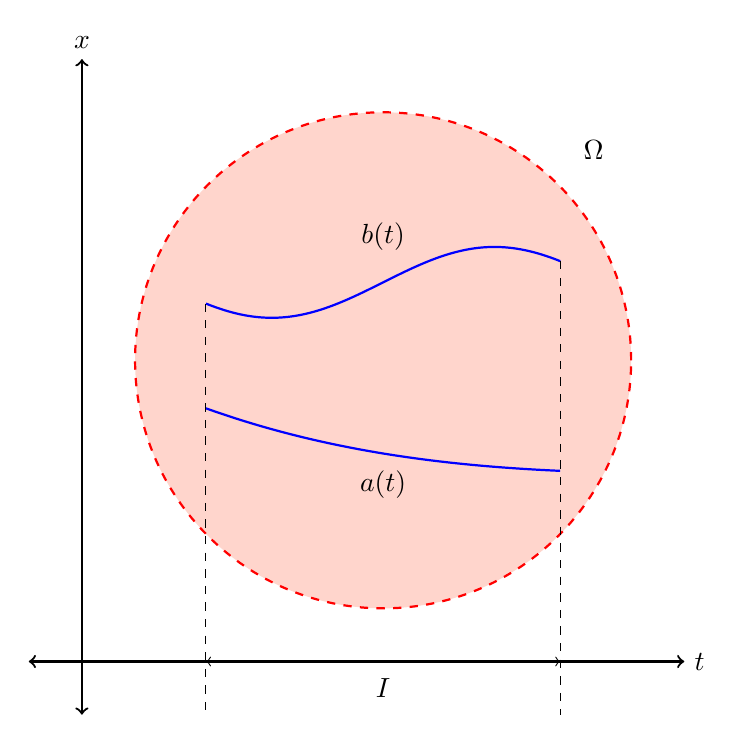
\begin{tikzpicture}[scale=0.9]
        \def\omgr{3.5}
        \def\omgm{0.75}
        \def\dom{-\omgr + 1: \omgr - 1}
        \def\b(#1){1.1+0.5 * sin((#1) r)}
        \def\a(#1){-(0.001*(#1-5.4)^2 +0.002*(#1-5.4)^3)-1.6}
        \filldraw[fill=Coral1!30, draw=red, dashed, thick] (0,0) circle (\omgr);
        \node at (\omgr * 1.2 * 0.7071, \omgr * 1.2 * 0.7071) {$\Omega$};
        \draw[blue, thick, domain=\dom, samples=100] plot (\x,{\b(\x)});
        \draw[blue, thick, domain=\dom, samples=100] plot (\x,{\a(\x)});
        \draw[<->, thick] (-\omgr - 2 *\omgm,-\omgm - \omgr) -- (\omgr + \omgm,-\omgm - \omgr) node[right] {$t$};
        \draw[<->, thick] (-\omgr - \omgm, -2 * \omgm - \omgr) -- (-\omgm - \omgr,\omgr + \omgm) node[above] {$x$};
        \node at (0, 0.5*\omgr) {$b(t)$};
        \node at (0, -0.5*\omgr) {$a(t)$};
        \draw[-, dashed, black] (-\omgr + 1, {\b(-\omgr + 1)}) -- (-\omgr + 1, -\omgr - 2*\omgm);
        \draw[-, dashed, black] (\omgr - 1, {\b(\omgr - 1)}) -- (\omgr - 1, -\omgr - 2*\omgm);
        \draw[<->, black] (-\omgr + 1, -\omgr - \omgm) -- (\omgr - 1, -\omgr - \omgm);
        \node at (0, -\omgr - 1.5*\omgm) {$I$};
    \end{tikzpicture}
\end{center}
Fijamos $t_0 \in I$ cualquiera. La función $F(t)$ ``recorre'' la variable $x$ integrando $f$ entre $a(t_0)$ y $b(t_0)$. Comencemos con la demostración.
\vspace{2mm} \newline \indent Sea $(t_n)_{n\in\N} \subseteq I \setminus \{t_0\}$ con $t_n \xrightarrow{n\to\infty} t_0$. Escribiremos la expresión de $F'(t_0)$ sin llegar todavía a tomar límites:
\begin{flalign*}
    &\frac{F(t_n) - F(t_0)}{t_n - t_0} = \frac{1}{t_n - t_0}\left(\int_{a(t_n)}^{b(t_n)}f(t_n, x)dx - \int_{a(t_0)}^{b(t_0)}f(t_0, x)dx\right) = \\[2ex]
    &\hspace{1mm} = \frac{1}{t_n - t_0} \left(\int_{a(t_n)}^{b(t_n)}f(t_n, x)dx - \int_{a(t_n)}^{b(t_0)}f(t_n, x)dx + \int_{a(t_n)}^{b(t_0)}f(t_n, x)dx - \right.\\[2ex]
    &\hspace{5ex} \left. - \int_{a(t_0)}^{b(t_0)}f(t_n, x)dx + \int_{a(t_0)}^{b(t_0)}f(t_n, x)dx - \int_{a(t_0)}^{b(t_0)}f(t_0, x)dx\right) = \\[2ex]
    &\hspace{1mm} = \frac{1}{t_n - t_0} \left(\int_{b(t_0)}^{b(t_n)}f(t_n,x)\,dx - \int_{a(t_0)}^{a(t_0)}f(t_n, x)\,dx - \int_{a(t_0)}^{b(t_0)}f(t_n,x)-f(t_0, x)\,dx\right) = (*)
\end{flalign*}
\vspace{2mm} Aplicando el Teorema del Valor Medio de Integración, existen $\xi_n \in I_{b(t_n), b(t_0)}$ y $\zeta_n \in I_{a(t_n), a(t_0)}$ tales que:
$$(*)= f(t_n, \xi_n) \cdot \frac{b(t_n)-b(t_0)}{t_n - t_0} - f(t_n, \zeta_n)\cdot \frac{a(t_n) - a(t_0)}{t_n - t_0} + \int_{a(t_0)}^{b(t_0)}\frac{f(t_n, x) - f(t_0, x)}{t_n - t_0} \,dx$$
\vspace{2mm} Por ser $a$  y $b$ derivables, tomando límites en los dos primeros sumandos:
$$\lim_{n\to\infty} f(t_n, \xi_n) \cdot \frac{b(t_n)-b(t_0)}{t_n - t_0} - f(t_n, \zeta_n)\cdot \frac{a(t_n) - a(t_0)}{t_n - t_0} = f\big(t_0, b(t_0)\big) \cdot b'(t_0) - f\big(t_0, a(t_0)\big) \cdot a'(t_0)$$
\vspace{2mm} Por el Teorema del Valor Medio de Derivación, sabemos que existe $\theta_n \in I_{t_n, t_0}$ tal que $\frac{f(t_n, x)- f(t_0, x)}{t_n - t_0} = \frac{\partial f}{\partial t}(\theta_n , x)$. Además, por ser $\Omega$ un abierto con $f$ continua en él, podemos afirmar que existen $\varepsilon > 0$, $\delta > 0$ tales que:
\begin{flalign*}
    &J := [t_0 - \delta, t_0 + \delta] \times [a(t_0) - \varepsilon, a(t_0) + \varepsilon] \subseteq \Omega \\
    &K := [t_0 - \delta, t_0 + \delta] \times [b(t_0) - \varepsilon, b(t_0) + \varepsilon] \subseteq \Omega
\end{flalign*}
Así, sea $t \in [t_0 - \delta, t_0 + \delta]$, tenemos que $a(t) \in [a(t_0) - \varepsilon, a(t_0) + \varepsilon]$ y $b(t) \in [b(t_0) - \varepsilon, b(t_0) + \varepsilon]$. Definimos $M := [t_0 - \delta, t_0 + \delta] \times [a(t_0) - \varepsilon, b_(t_0) + \varepsilon]$. Veamos qué papel juegan estos conjuntos en nuestro esquema anterior:
\vspace{6mm} \newline
\begin{minipage}{0.5\textwidth}
    \begin{center}
        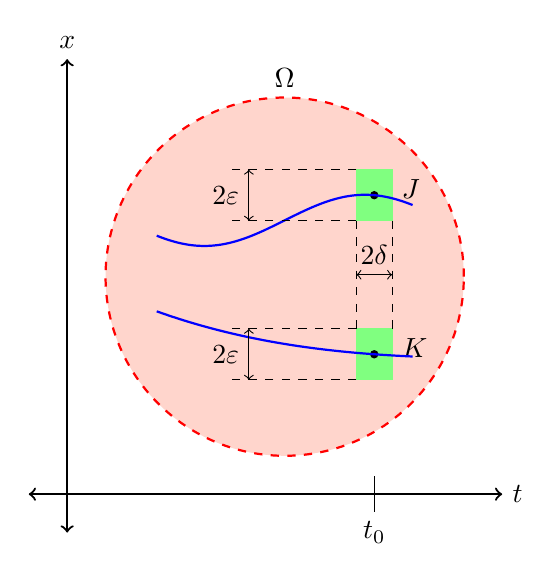
\begin{tikzpicture}[scale=0.65]
            \def\omgr{3.5}
            \def\omgm{0.75}
            \def\dom{-\omgr + 1: \omgr - 1}
            \def\t0{0.5*\omgr}
            \def\eps{0.5}
            \def\delt{0.35}
            \def\b(#1){1.1+0.5 * sin((#1) r)}
            \def\a(#1){-(0.001*(#1-5.4)^2 +0.002*(#1-5.4)^3)-1.6}
            \draw[<->, thick] (-\omgr - 2 *\omgm,-\omgm - \omgr) -- (\omgr + \omgm,-\omgm - \omgr) node[right] {$t$};
            \draw[<->, thick] (-\omgr - \omgm, -2 * \omgm - \omgr) -- (-\omgm - \omgr,\omgr + \omgm) node[above] {$x$};
            \filldraw[fill=Coral1!30, draw=red, dashed, thick] (0,0) circle (\omgr);
            \node[above, text=black] at (0, \omgr) {$\Omega$};        
            \filldraw[green!50] ({\t0 - \delt}, {\b(\t0) - \eps}) rectangle ({\t0 + \delt}, {\b(\t0) + \eps}) node[anchor=north west] {$\textcolor{black}{J}$};
            \filldraw[green!50] ({\t0 - \delt}, {\a(\t0) - \eps}) rectangle ({\t0 + \delt}, {\a(\t0) + \eps}) node[anchor=north west] {$\textcolor{black}{K}$};
            \filldraw[black] ({\t0}, {\b(\t0)}) circle (2pt);
            \filldraw[black] ({\t0}, {\a(\t0)}) circle (2pt);
            \draw[blue, thick, domain=\dom, samples=100] plot (\x,{\b(\x)});
            \draw[blue, thick, domain=\dom, samples=100] plot (\x,{\a(\x)});
            \draw[dashed] ({\t0 + \delt}, {\b(\t0) - \eps}) -- ({\t0 + \delt}, {\a(\t0) + \eps});
            \draw[dashed] ({\t0 - \delt}, {\b(\t0) - \eps}) -- ({\t0 - \delt}, {\a(\t0) + \eps});
            \draw[<->] ({\t0 - \delt},{0.5*(\b(\t0) + \a(\t0))}) -- ({\t0 + \delt},{0.5*(\b(\t0) + \a(\t0))}) node[midway,above] {$2\delta$};
            \draw[dashed] ({\t0 - \delt}, {\b(\t0) - \eps}) -- ({\t0 - 8*\delt}, {\b(\t0) - \eps});
            \draw[dashed] ({\t0 - \delt}, {\b(\t0) + \eps}) -- ({\t0 - 8*\delt}, {\b(\t0) + \eps});
            \draw[<->] ({\t0 - 7* \delt},{\b(\t0) + \eps}) -- ({\t0 - 7 *\delt},{\b(\t0) - \eps}) node[midway,left] {$2\varepsilon$};
            \draw[dashed] ({\t0 - \delt}, {\a(\t0) - \eps}) -- ({\t0 - 8*\delt}, {\a(\t0) - \eps});
            \draw[dashed] ({\t0 - \delt}, {\a(\t0) + \eps}) -- ({\t0 - 8*\delt}, {\a(\t0) + \eps});
            \draw[<->] ({\t0 - 7* \delt},{\a(\t0) + \eps}) -- ({\t0 - 7 *\delt},{\a(\t0) - \eps}) node[midway,left] {$2\varepsilon$};
            \draw[-] (\t0, -\omgr - \omgm + \delt) -- (\t0, -\omgr - \omgm - \delt) node[below] {$t_0$};
        \end{tikzpicture}
    \end{center}
\end{minipage}
\begin{minipage}{0.5\textwidth}    
    \begin{center}
    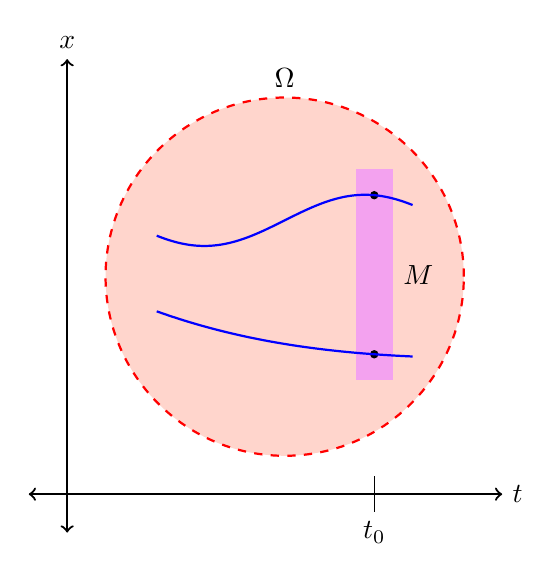
\begin{tikzpicture}[scale=0.65]
        \def\omgr{3.5}
        \def\omgm{0.75}
        \def\dom{-\omgr + 1: \omgr - 1}
        \def\t0{0.5*\omgr}
        \def\eps{0.5}
        \def\delt{0.35}
        \def\b(#1){1.1+0.5 * sin((#1) r)}
        \def\a(#1){-(0.001*(#1-5.4)^2 +0.002*(#1-5.4)^3)-1.6}
        \draw[<->, thick] (-\omgr - 2 *\omgm,-\omgm - \omgr) -- (\omgr + \omgm,-\omgm - \omgr) node[right] {$t$};
        \draw[<->, thick] (-\omgr - \omgm, -2 * \omgm - \omgr) -- (-\omgm - \omgr,\omgr + \omgm) node[above] {$x$};
        \filldraw[fill=Coral1!30, draw=red, dashed, thick] (0,0) circle (\omgr);
        \node[above, text=black] at (0, \omgr) {$\Omega$};        
        \filldraw[Orchid2!70] ({\t0 - \delt}, {\a(\t0) - \eps}) rectangle ({\t0 + \delt}, {\b(\t0) + \eps}) node[midway, right, xshift={20*\delt}] {$\textcolor{black}{M}$};
        \filldraw[black] ({\t0}, {\b(\t0)}) circle (2pt);
        \filldraw[black] ({\t0}, {\a(\t0)}) circle (2pt);
        \draw[blue, thick, domain=\dom, samples=100] plot (\x,{\b(\x)});
        \draw[blue, thick, domain=\dom, samples=100] plot (\x,{\a(\x)});       
        \draw[-] (\t0, -\omgr - \omgm + \delt) -- (\t0, -\omgr - \omgm - \delt) node[below] {$t_0$};
    \end{tikzpicture}
    \end{center}
\end{minipage}
\vspace{6mm} \newline \indent Tenemos que $M$ es compacto por definición. Además, como $f \in \mathcal{C}^1(\Omega)$ por hipótesis, podemos garantizar que:
$$\exists \hspace{1mm} m := \max \left\{\left|\frac{\partial f}{\partial t}(x, t)\right| : (x,t) \in M\right\} $$
De este modo, estamos en condiciones de aplicar el \hyperref[result:2.2.7]{Teorema de la Convergencia Dominada}. Por todo lo anterior,
\begin{flalign*}
    \lim_{n\to\infty}& f(t_n, \xi_n) \cdot \frac{b(t_n)-b(t_0)}{t_n - t_0} - f(t_n, \zeta_n)\cdot \frac{a(t_n) - a(t_0)}{t_n - t_0} + \int_{a(t_0)}^{b(t_0)}\frac{f(t_n, x) - f(t_0, x)}{t_n - t_0}\,dx = \\[2ex]
    &= f\big(t_0, b(t_0)\big) \cdot b'(t_0) - f\big(t_0, a(t_0)\big) \cdot a'(t_0) + \int_{a(t_0)}^{b(t_0)} \frac{\partial f}{\partial t}(x, t_0) \,dx
\end{flalign*}

\newpage
\chapter{Cálculo de la integral de Lebesgue en \texorpdfstring{$\R^N$}{R\^N}}
\result{Notación y conceptos iniciales}
\hspace{3mm} $\R^{p+q} = \R^p \times \R^q$ con $p,q\in\N$. Así, si $x \in \R^p$ con $y \in \R^q$; entonces, $(x,y) \in \R^{p+q}$.
\newline \indent Sea $E \subseteq \R^{p+q}$, sea $x \in \R^p$. Definimos la sección de $E$ por $x$ como el conjunto:
$$E_x = \Big\{y \in \R^q : (x,y) \in E\Big\}$$
De manera similar, sea $y \in \R^{q}$, definimos la sección de $E$ por $y$ como:
$$E_y = \Big\{x \in \R^p : (x,y) \in E\Big\}$$
\indent Sea $f: \R^{p+q} \longrightarrow \overline{\R}$ \hspace{1mm} $(x,y) \longmapsto f(x,y)$. Definimos la sección de $f$ por $x \in \R^p$ y la sección de $f$ por $y \in \R^q$ (respectivamente) como las dos siguientes funciones: \\[-2.5ex]
\begin{minipage}{0.5\textwidth}
    \begin{flalign*}
        f_x :& \R^q \longrightarrow \overline{\R}\\
        &x \longmapsto f(x,y)
    \end{flalign*}
\end{minipage}
\begin{minipage}{0.5\textwidth}
    \begin{flalign*}
        f_y :& \R^p \longrightarrow \overline{\R}\\
        &y \longmapsto f(x,y)
    \end{flalign*}
\end{minipage}

\vspace{6mm} \result{Propiedades de las secciones}
\hspace{3mm} Sea $f : \R{p+q} \longrightarrow \overline{\R}$. Sean $\{E\}\cup\{E^i\}_{i\in\N} \subseteq \R^{p+q}$. Sean $x \in \R^p, y \in \R^q$. Entonces, se cumplen los siguientes enunciados:
\\[2ex]
\begin{minipage}{0.5\textwidth}
    \begin{enumerate}[label=\roman*)]
        \item $(f^+)_x = (f_x)^+$
        \item $(f^-)_x = (f_x)^-$
        \item $(\smallcup_{i\in\N}E^i)_x = \smallcup_{i\in\N}E^i_x$
        \item $(\smallcap_{i\in\N}E^i)_x = \smallcap_{i\in\N}E^i_x$
        \item $(\R^{p+q}\setminus E)_x = \R^q \setminus E_x$.
    \end{enumerate}
\end{minipage}
\begin{minipage}{0.5\textwidth}
    \begin{enumerate}[label=\roman*')]
        \item $(f^+)_y = (f_y)^+$
        \item $(f^-)_y = (f_y)^-$
        \item $(\smallcup_{i\in\N}E^i)_y = \smallcup_{i\in\N}E^i_y$
        \item $(\smallcap_{i\in\N}E^i)_y = \smallcap_{i\in\N}E^i_y$
        \item $(\R^{p+q}\setminus E)_y = \R^p \setminus E_y$.
    \end{enumerate}
\end{minipage}
\\[4ex] \dem Las demostraciones $(*')$ son análogas al resto.
\vspace{2mm} \newline $\romannumeral 1)$ $(f_x)^+(y) = \max\{f_x(y),0\} = \max\{f(x,y), 0\} = f^+(x,y) = (f^+)_x(y)$.
\vspace{2mm} \newline $\romannumeral 2)$ $(f_x)^-(y) = \max\{-f_x(y),0\} = \max\{-f(x,y), 0\} = f^-(x,y) = (f^-)_x(y)$.
\vspace{6mm} \newline $\romannumeral 3)$ Veamos que $(\smallcup_{i\in\N}E^i)_y = \smallcup_{i\in\N}E^i_y$ por doble contenido:
\begin{tcolorbox}[Subset-contingency]
    $\subseteq$ \hspace{2mm} Si $y \in (\smallcup_{i\in\N}E^i)_x$, tenemos $(x,y) \in \smallcup_{i\in\N}E^n$ luego $\exists \hspace{1mm} j \in \N$ tal que $(x,y) \in E_j$. 
\end{tcolorbox}
Por tanto, $y \in E^j_x \subseteq \smallcup_{i\in\N}E^i_x$.
\vspace{2mm}
\begin{tcolorbox}[Subset-contingency]
    $\supseteq$ \hspace{2mm} Si $y \in \smallcup_{i\in\N}E^i_x$, tenemos $\exists \hspace{1mm} j \in \N$ tal que $y \in E^j_x$. Así, $(x,y) \in E^j \subseteq \smallcup_{i\in\N} E^i$.
\end{tcolorbox}
Por tanto, $y \in (\smallcup_{i\in\N} E^i)_x$.

\vspace{8mm} $\romannumeral 4)$ Lo veremos por la definición del conjunto. Como $y$ es un punto fijo de $\R^q$ (dado por el enunciado), usaremos $z$ como variable genérica de $\R^q$.
\begin{flalign*}
    (\smallcap_{i\in\N}E^i)_x = \Big\{z \in \R^q : (x,z) \in \smallcap_{i\in\N}E^i\Big\} = \bigcap_{i\in\N}\Big\{z \in \R^q : (x,z) \in E^i\Big\} = \smallcap_{i\in\N}E^i_x
\end{flalign*}

\vspace{8mm} \noindent $\romannumeral 5)$ Veamos que $(\R^{p+q}\setminus E)_x = \R^q \setminus E_x$ por doble contenido:
\begin{tcolorbox}[Subset-contingency]
    $\subseteq$ \hspace{2mm} Si $y \in (\R^{p+q}\setminus E)_x$, tenemos $(x,y) \in \R^{p+q} \setminus E$ luego $(x,y) \notin E$. 
\end{tcolorbox}
Por tanto, $y \notin \{z \in \R^q : (x,z) \in E\} = E_x$ luego $y \in \R^q \setminus E_x$.
\vspace{2mm}
\begin{tcolorbox}[Subset-contingency]
    $\subseteq$ \hspace{2mm} Si $y \in \R^{q}\setminus E_x$, tenemos $y \notin \{z \in \R^q : (x,y) \in E\} = E_x$. 
\end{tcolorbox}
Por tanto, $(x,y) \notin E$ luego $(x,y) \in \R^{p+q} \setminus E$ y por tanto $y \in (\R^{p+q} \setminus E)_x$.

\vspace{6mm} \noindent $\nota$ A partir de los apartados $(iii)$, $(iv)$, $(iii')$ y $(iv')$ se deducen los siguientes para $E, F \in \R^{p+q}$ cualesquiera:
\begin{align*}
    v) \hspace{2mm}(E \setminus F)_x = E_x \setminus F_x &&
    v') \hspace{2mm}  (E \setminus F)_y = E_y \setminus F_y
\end{align*}

\newpage
\result{Teorema de anomalías de conjuntos medibles}
\hspace{3mm} Sea $E \in \mathfrak{M}_{p+q}$. Se cumplen los siguientes enunciados: \\[4ex]
\begin{minipage}{0.5\textwidth}
    \begin{enumerate}[leftmargin=0mm, label=\alph*)]
        \item $\exists \hspace{1mm} A \in \mathfrak{M}_p$ con $\mu_p(A) = 0$ que verifica: \\[-3ex]
        $$\forall \hspace{1mm} x \in \R^p \setminus A : E_x \in \mathfrak{M}_q$$
        \item La siguiente función es $\mu_p$-medible: \\[-6ex]
        \begin{align*}
            \varphi : \R^p \setminus A \to \R&& x \mapsto \varphi(x) = \mu_q(E_x)
        \end{align*}
        \item Medida por secciones en $x$: \\[-2ex]
        $$\int_{\R^p \setminus A}\varphi(x)\,d\mu_p(x) = \mu_{p+q}(E)$$
    \end{enumerate}
\end{minipage}
\begin{minipage}{0.5\textwidth}
    \begin{enumerate}[leftmargin=7mm, rightmargin=0mm, label=\alph*')]
        \item $\exists \hspace{1mm} B \in \mathfrak{M}_q$ con $\mu_p(A) = 0$ que verifica: \\[-3ex]
        $$\forall \hspace{1mm} y \in \R^q \setminus B : E_y \in \mathfrak{M}_p$$
        \item La siguiente función es $\mu_q$-medible: \\[-6ex]
        \begin{align*}
            \psi : \R^q \setminus B \to \R&& y \mapsto \psi(y) = \mu_p(E_y)
        \end{align*}
        \item Medida por secciones en $y$: \\[-2ex]
        $$\int_{\R^q \setminus B}\psi(y)\,d\mu_q(y) = \mu_{p+q}(E)$$
    \end{enumerate}
\end{minipage}
\\[6ex] \dem Veremos solo los tres primeros apartados (los apartados' son análogos). Iremos estructurando la demostración por casos de complejidad incremental.

\vspace{6mm} $\romannumeral 1)$ Para $E$ un cubo acotado. Podemos expresar $E = I \times J$ con $I, J$ cubos acotados de $\R^p$ y $\R^q$, respectivamente.
\begin{adjustwidth}{0.07\textwidth}{}
    \vspace{-3ex}
    \begin{flalign*}
        \text{a) Sea } x\in\R^p, E_x = \begin{cases}
            J &\text{si } x \in I \\
            \varnothing &\text{si } x \notin I
        \end{cases} \hspace{4mm} \text{ En cualquier caso, }E_x \in \mathfrak{M}_q&&
    \end{flalign*}
    \\[-3ex]
    \begin{flalign*}
        \text{b) }\varphi(x) = \left.\begin{cases}
        \mu_q(J) &\text{ si } x \in I\\
        \mu_q(\varnothing) &\text{ si } x \notin I
        \end{cases}\right\} = \mu_q(J) \cdot X_I(x) \hspace{2mm} \text{ que es } \mu_p\text{-medible}.&&
    \end{flalign*}
    \begin{flalign*}
        \text{c) } \int_{\R^p}\varphi(x)\,d\mu_p(x) = \mu_q(J) \cdot \int_{\R^p}X_I(x)\,d\mu_p(x) = \mu_p(I) \cdot \mu_q(J) = \mu_{p+q}(E)&&
    \end{flalign*}
\end{adjustwidth}

\vspace{6mm} $\romannumeral 2)$ Para $E$ un abierto acotado. Sabemos que podemos expresar $E = \smallcup_{n\in\N}I^n$ donde los $I_n$ son cubos diádicos disjuntos. Aplicando el apartado anterior a cada uno de ellos, sabemos que para $x \in \R^p$ cualquiera, se tiene:
\\[-3ex]  %TODO referenciar resultado cubos diádicos
\begin{align*}
    I^n_x \in \mathfrak{M}_q &&
    \varphi_n(x) = \mu_q(I_x^n) \hspace{2mm} \mu_p\text{-medible} &&
    \int_{\R^p}\varphi_n(x)\,d\mu_p(x) = \mu_{p+q}(I^n)
\end{align*}
Veamos cómo demostrar el apartado $(\romannumeral 2)$ en base a esta información:
\begin{adjustwidth}{0.07\textwidth}{}
    \vspace{-5ex}
    \begin{flalign*}
        \text{a) }E_x = (\smallcup_{n\in\N}I^n)_x \overset{\hyperref[result:2.4.2]{2.4.2}}{=} \smallcup_{n\in\N} I^n_x \in \mathfrak{M}_q \hspace{4ex} \text{ Consideramos } A = \varnothing.&&
    \end{flalign*}
    \\[-8ex]
    \begin{flalign*}
        %TODO referenciar resultado de límite medible
        \text{b) }\varphi(x) = \mu_q(E_x) =\mu_q \big(\smallcup_{n\in\N}I^n_x\big)  =\sum_{n=1}^{\infty}\mu_q(I^n_x) = \lim_{n\to \infty} \sum_{k=1}^{n}\varphi_k(x) \hspace{2ex} \mu_q\text{-medible}.&&
    \end{flalign*}
    \\[-6ex]
    \begin{flalign*}
        \text{c) }& \int_{\R^p}\varphi(x)\,d\mu_p(x) = \int_{\R^p}\sum_{n=1}^{^\infty}\varphi_n(x)\,d\mu_p(x) \overset{\hyperref[result:2.1.10]{TCM}}{=} \sum_{n=1}^{\infty} \int_{\R^p}\varphi_n\,d\mu_p(x) =&& \\
        &= \sum_{n=1}^{\infty} \mu_{p+q}(I^n) = \mu_{p+q}\big(\smallcup_{n\in\N}I^n\big) = \mu_{p+q}(E)
    \end{flalign*}
\end{adjustwidth}

\vspace{6mm} $\romannumeral 3)$ Para $E = \smallcap_{n\in\N}O^n$ intersección de abiertos decrecientes. Aplicando el apartado anterior, sabemos que para $x \in \R^p$ cualquiera se cumple:
\begin{align*}
    O^n_x \in \mathfrak{M}_q &&
    \varphi_n(x) = \mu_q(O_x^n) \hspace{2mm} \mu_p\text{-medible} &&
    \int_{\R^p}\varphi_n(x)\,d\mu_p(x) = \mu_{p+q}(O^n)
\end{align*}
Demostraremos el apartado $(\romannumeral 3)$ con esta información:
\begin{adjustwidth}{0.07\textwidth}{}
    \vspace{-5ex}
    \begin{flalign*}
        \text{a) }E_x = (\smallcap_{n\in\N}O^n)_x \overset{\hyperref[result:2.4.2]{2.4.2}}{=} \smallcap_{n\in\N} O^n_x \in \mathfrak{M}_q \hspace{4ex} \text{ Consideramos } A = \varnothing.&&
    \end{flalign*}
    \\[-8ex]
    \begin{flalign*}
        %TODO referenciar resultado de límite por abajo de la medida
        \text{b) }\varphi(x) = \mu_q(E_x) =\mu_q \big(\smallcap_{n\in\N}O^n_x\big)  = \lim_{n\to\infty}\mu_q(O^n_x) = \lim_{n\to\infty}\varphi_n(x) \hspace{4mm} \mu_q\text{-medible}&&
    \end{flalign*}
    \\[-6ex]
    \begin{flalign*}
        \text{c) }& \int_{\R^p}\varphi(x)\,d\mu_p(x) = \int_{\R^p}\lim_{n\to\infty}\varphi_n(x)\,d\mu_p(x) \overset{\hyperref[result:2.2.7]{TCD \hspace{1mm}\varphi_1}}{=} \lim_{n\to\infty} \int_{\R^p}\varphi_n\,d\mu_p(x) =&& \\
        &= \lim_{n\to\infty}\mu_{p+q}(O^n) = \mu_{p+q}(E)
    \end{flalign*}
\end{adjustwidth}

%TODO referenciar
\vspace{6mm} $\romannumeral 4) \hspace{2mm} E \in \mathfrak{M}_{p+q}$ con $\mu_{p+q}(E) = 0$. Por la caracterización topológica de los conjuntos medibles, sabemos que existen $\{O^n\}_{n\in\N} \subseteq \tau_{\R^{p+q}}$ con $E \subseteq O^{n+1} \subseteq O^n$ y tales que $\mu_{p+q}(O^n) \xrightarrow{n\to\infty}0$. De este modo, tenemos $E \subseteq N:= \smallcap_{n\in\N}O^n \in \mathfrak{M}_{p+q}$. Aplicando el apartado anterior a $N$, tenemos que para $x\in\R^p$ se cumple:
\vspace{-1.5ex}
\begin{align*}
    N_x \in \mathfrak{M}_q &&
    \varphi_1(x) = \mu_q(N_x) \hspace{2mm} \mu_p\text{-medible} &&
    \int_{\R^p}\varphi_1(x)\,d\mu_p(x) = \mu_{p+q}(N) = 0
\end{align*}

%TODO referenciar integral nula de función no negativa
\vspace{-1.5ex} \noindent Al ser $\varphi_1$ no negativa con integral nula, sabemos que $\varphi_1 \overset{\mu-a.e.}{=} 0$ luego $\exists \hspace{1mm} A \in \mathfrak{M}_p$ con $\mu_p(A) = 0$ tal que $\{x \in \R^p : \varphi_1(x) \neq 0\} \subseteq A$. Sea este el conjunto de anomalías para este apartado, dado $x \in \R^p \setminus A$, se cumple:
\begin{adjustwidth}{0.07\textwidth}{}
    \vspace{-5ex}
    \begin{flalign*}
        \text{a) }E_x \subseteq N_x \text{ con } \mu_q(E_x) \leq \mu_q(N_x) = \varphi_1(x) = 0 \text{ luego } E_x \in \mathfrak{M}_q.&&
    \end{flalign*}
    \\[-10ex]
    \begin{flalign*}
        \text{b) }\varphi(x) = \mu_q(E_x) =0 \hspace{4mm} \mu_q\text{-medible trivialmente}.&&
    \end{flalign*}
    \\[-9ex]
    \begin{flalign*}
        \text{c) }& \int_{\R^p \setminus A}\varphi(x)\,d\mu_p(x) = \int_{\R^p \setminus A}0\,d\mu_p(x) = 0 = \mu_{p+q}(E)&&
    \end{flalign*}
\end{adjustwidth}

%TODO referenciar expresión de medibles Lebesgue según borelianos
\vspace{6mm} $\romannumeral 5)$ Para $E \in \mathfrak{M}_{p+q}$ acotado. Por ser medible, $E = G\setminus N$, donde $G$ es una intersección de abiertos decrecientes y $N$ es un conjunto de medida nula. Al ser $E$ acotado, también ha de serlo $G$, luego estamos en condiciones de aplicarle el apartado $(\romannumeral 3)$. Así, para $x \in \R^p$ se cumple:
\vspace{-2ex}
\begin{align*}
    G_x \in \mathfrak{M}_q &&
    \varphi_1(x) = \mu_q(G_x) \hspace{2mm} \mu_p\text{-medible} &&
    \int_{\R^p}\varphi_1(x)\,d\mu_p(x) = \mu_{p+q}(G)
\end{align*}

\vspace{-1.5ex} \noindent Aplicando ahora el apartado $(\romannumeral 4)$ a $N$, para $x \in \R^p \setminus A$ se tiene:
\vspace{-1ex}
\begin{align*}
    N_x \in \mathfrak{M}_q &&
    \varphi_2(x) = \mu_q(N_x) \hspace{2mm} \mu_p\text{-medible} &&
    \int_{\R^p \setminus A}\varphi_2(x)\,d\mu_p(x) = \mu_{p+q}(N)
\end{align*}

\vspace{-1.5ex} \noindent Consideramos este conjunto $A$. Así, dado $x \in \R^p \setminus A$, tenemos:
\begin{adjustwidth}{0.07\textwidth}{}
    \vspace{-5ex}
    \begin{flalign*}
        \text{a) }E_x \subseteq N_x \text{ con } \mu_q(E_x) \leq \mu_q(N_x) = \varphi_1(x) = 0 \text{ luego } E_x \in \mathfrak{M}_q.&&
    \end{flalign*}
    \\[-10ex]
    \begin{flalign*}
        \text{b) }\varphi(x) = \mu_q(E_x) = \mu_q(G_x) - \mu_q(N_x) = \varphi_1(x) - \varphi_2(x) \hspace{4mm} \mu_q\text{-medible}.&&
    \end{flalign*}
    \\[-8ex]
    \begin{flalign*}
        \text{c) }& \int_{\R^p \setminus A}\varphi(x)\,d\mu_p(x) = \int_{\R^p \setminus A}0\,d\mu_p(x) = 0 = \mu_{p+q}(E)&&
    \end{flalign*}
\end{adjustwidth}

%TODO referenciar conjuntos medibles según borelianos
\vspace{6mm} $\romannumeral 6)$ $E \in \mathfrak{M}_{p+q}$ (caso general). Definimos $E^n = E \cap [-n,n]^N$. De este modo, es claro que $E = \smallcup_{n\in\N}E^n$ y que todos los $E^n$ son acotados. Aplicando el apartado ($\romannumeral 5$) a cada uno de ellos, tenemos que para $x \in \R^p \setminus A^n$ se cumple:
\begin{align*}
    E^n_x \in \mathfrak{M}_q &&
    \varphi_n(x) = \mu_q(E^n_x) \hspace{2mm} \mu_p\text{-medible} &&
    \int_{\R^p \setminus A^n}\varphi_1(x)\,d\mu_p(x) = \mu_{p+q}(E^n)
\end{align*}
Consideramos el conjunto de anomalías $A := \smallcup_{n\in\N} A^n$ aplicando la subaditividad de la medida, es claro que $\mu_{p+q}(A) = 0$. Sea $x \in R^p \setminus A$, se cumple:
\begin{adjustwidth}{0.07\textwidth}{}
    \vspace{-5ex}
    \begin{flalign*}
        \text{a) }E_x = \smallcup_{i\in\N}\underbracket{E^n_x}_{\in \mathfrak{M}_q} \in \mathfrak{M}_q &&
    \end{flalign*}
    \\[-10ex]
    \begin{flalign*}
        \text{b) }\varphi(x) = \mu_q(E_x) =  \lim_{n\to\infty}\mu_q(E^n_x) = \lim_{n\to\infty}\varphi_n(x)\hspace{4mm} \mu_q\text{-medible}.&&
    \end{flalign*}
    \\[-9ex]
    \begin{flalign*}
        \text{c) }& \int_{\R^p \setminus A}\varphi(x)\,d\mu_p(x) = \int_{\R^p \setminus A} \lim_{n\to\infty}\varphi_n(x)\,d\mu_p(x) \overset{\hyperref[result:2.1.10]{TCM}}{=} \lim_{n\to\infty} \int_{R^p \setminus A}\varphi_n(x)\,d\mu = &&\\[2ex]
         &= \lim_{n \to \infty} \mu_{p+q}(E^n) = \mu_{p+q}(E)
    \end{flalign*}
\end{adjustwidth}

\vspace{6mm}
\result{Teorema de Tonelli}
\hspace{3mm} Sea $f : \R^{p+q} \longrightarrow [0,+\infty]$ una función $\mu_{p+q}$-medible. Tenemos:
\\[3ex]
\begin{minipage}{0.5\textwidth}
    \begin{enumerate}[leftmargin=0mm, label=\alph*)]
        \item $\exists A \in \mathfrak{M}_q$ con $\mu_p(A)=0$ que verifica: \\[-3ex] 
        $$\forall \hspace{1mm} x \in \R^p \setminus A \hspace{1mm} f_x \text{ es } \mu_q\text{-medible}$$
        \item La siguiente función $\varphi : \R^p \setminus A \to [0,+\infty]$ \\[-6ex]
        \begin{align*}
            x \mapsto \int_{\R^q}f_x(y)\,d\mu_q(y) && \text{ es }\mu_q\text{-medible}
        \end{align*}
        \item Integración por secciones: \\[-2.5ex]
        $$\hspace{-5ex} \int_{\R^p \setminus A} \hspace{-3mm} \varphi(x)\,d\mu_p(x) = \int_{\R^{p+q}} \hspace{-3mm} f(x,y)\,d\mu_{p+q}(x,y)$$
    \end{enumerate}
\end{minipage}
\begin{minipage}{0.55\textwidth}
    \begin{enumerate}[leftmargin=8mm, rightmargin=-2mm, label=\alph*')]
        \item $\exists B \in \mathfrak{M}_p$ con $\mu_p(B)=0$ que verifica: \\[-3ex] 
        $$\forall \hspace{1mm} y \in \R^q \setminus B \hspace{1mm} f_y \text{ es } \mu_p\text{-medible}$$
        \item La siguiente función $\psi : \R^q \setminus B \to [0,+\infty]$ \\[-6ex]
        \begin{align*}
            y \mapsto \int_{\R^p}f_y(x)\,d\mu_p(x) && \text{ es }\mu_p\text{-medible}
        \end{align*}
        \item Integración por secciones: \\[-2.5ex]
        $$\int_{\R^q \setminus B} \hspace{-3mm} \varphi(y)\,d\mu_q(y) = \int_{\R^{p+q}} \hspace{-3mm} f(x,y)\,d\mu_{p+q}(x,y)$$
    \end{enumerate}
\end{minipage}
Por tanto, ha de cumplirse:
$$ \int_{\R^p}\left(\int_{\R^q}f(x,y)\,d\mu_q(y)\right)\,d\mu_p(x) = \int_{\R^{p+q}} \hspace{-4mm} f(x,y)\,d\mu_{p+q}(x,y) = \int_{\R^q}\left(\int_{\R^p}f(x,y)\,d\mu_p(x)\right)\,d\mu_q(y)$$

\vspace{2mm} \dem Al igual que con el caso anterior; dividiremos la demostración en casos, y no se demostrarán los apartados' al ser análogos.
\vspace{2mm} \newline $\romannumeral 1)$ Consideramos $f = X_E$ para cierto $E \in \mathfrak{M}_{p+q}$. Se corresponde con el \hyperref[result:2.4.3]{teorema anterior}. Así, para el correspondiente conjunto de anomalías $A \in \mathfrak{M}_{p+q}$ con $\mu_{p+q}(A) = 0$ fijado, tenemos:
\begin{adjustwidth}{0.07\textwidth}{}
    \vspace{-4ex}
    \begin{flalign*}
        \text{a) }f_x = (X_E)_x = x_{E_x} \mu_q\text{-medible al ser }E_x \in \mathfrak{M}_q&&
    \end{flalign*}
    \\[-8ex]
    \begin{flalign*}
        \text{b) }\varphi(x) = \int_{\R^q}X_{E_x}(y)\,d\mu_q(y) = \mu_q(E_x) \text{ medible por el \hyperref[result:2.4.3]{teorema anterior}}&&
    \end{flalign*}
    \\[-8ex]
    \begin{flalign*}
        \text{c) }\int_{\R^p \setminus A}\varphi(x)\,d\mu_p(x) = \mu_{p+q}(E) = \int_{\R^{p+q}}\underbrace{X_{E}(x,y)}_{f(x,y)}\,d\mu_{p+q}(x,y) &&
    \end{flalign*}
\end{adjustwidth}

\vspace{6mm} \indent $\romannumeral 2)$ Sea $f = \displaystyle \sum_{i=1}^{k} \lambda_i \cdot X_{E^i}$ función simple y medible dada por su expresión canónica. Aplicando el apartado anterior a cada $E^i$, tenemos que $\exists \hspace{1mm} A_i \in \mathfrak{M}_{p+q}$ con $\mu_{p+q}(A_i) = 0$ tal que $\forall \hspace{1mm} x \in \R^p \setminus A_i$ se cumple:
\begin{align*}
    (X_{E^i})_x \hspace{1mm} \mu_q\text{-medible} &&
    \varphi_i(x) = \int_{\R^q}X_{E^i_x}(y)\,d\mu_q(y) \text{ es }\mu_q\text{-medible}
\end{align*}
$$\int_{\R^p \setminus A_i}\varphi_i(x)\,d\mu_p(x) = \int_{\R^{p+q}}X_{E^i}(x,y)\,d\mu_{p+q}(x,y)$$

\vspace{4mm} Consideramos $A = \smallcup_{i\in\N}A_i \in \mathfrak{M}_{p}$, que cumple $\mu_p(A) = 0$ por subaditividad. Así, dado $x \in \R^p \setminus A$, se cumple:
\vspace{-5ex}
\begin{adjustwidth}{0.07\textwidth}{}
    \begin{flalign*}
        \text{a) } f_x = \sum_{i=1}^{k} \lambda_i \cdot \underbracket{X_{E^i}}_{\mu_q\text{-medible}} \hspace{1mm} \mu_q \text{-medible}&&
    \end{flalign*}
    \\[-6ex]
    \begin{flalign*}
        \text{b) } \varphi(x)& = \int_{\R^q}\sum_{i=1}^{k}\lambda_i \cdot X_{E^i_x}(y)\,d\mu_q(y)  = \sum_{i=1}^{k}\lambda_i \cdot \left(\int_{\R^q}X_{E^i_x}(y)\,d\mu_q(y)\right) =&& \\[1ex]
        &= \sum_{i=1}^k \lambda_i \cdot \underbracket{\varphi_i(x)}_{\mu_p \text{-medible}} \hspace{2mm} \mu_p \text{-medible}
    \end{flalign*}
    \\[-6ex]
    \begin{flalign*}
        \text{c) } \int_{\R^p \setminus A}&\varphi(x)\,d\mu_p(x) = \sum_{i=1}^{k} \lambda_i \cdot \int_{\R^p \setminus A}\varphi_i(x)\,d\mu_p(x) = \sum_{i=1}^{k}\lambda_i \cdot \int_{\R^p \setminus A_i}\varphi_i(x)\,d\mu_p(x) =&&\\
        =& \sum_{i=1}^k \lambda_i \cdot \mu_{p+q}(E^i) = \int_{\R^{p+q}}f(x,y)\,d\mu_{p+q}(x,y)
    \end{flalign*}
\end{adjustwidth}

%TODO referenciar funciones medibles como límite de simples
\vspace{6mm} $\romannumeral 3)$ $f \mu_{p+q}$-medible (caso general). Sabemos que existe una sucesión de funciones medibles y simples $(s_n)_{n\in\N}$ tales que $0\leq s_n \leq s_{n+1} \leq f$ que converge puntualmente a $f$. Aplicando el apartado anterior a cada $s_n$, tenemos que $\exists A_n \in \mathfrak{M}_p$ con $\mu_p(A_n) = 0$ tal que para cualquier $x \in \R^p \setminus A_n$ se cumple:
\begin{align*}
    (s_n)_x \hspace{1mm} \mu_q\text{-medible} &&
    \varphi_n(x) = \int_{\R^q}s_{n_x}(y)\,d\mu_q(y) \text{ es }\mu_q\text{-medible}
\end{align*}
$$\int_{\R^p \setminus A_n}\varphi_n(x)\,d\mu_p(x) = \int_{\R^{p+q}}s_n(x,y)\,d\mu_{p+q}(x,y)$$

\vspace{4mm} Consideramos $A = \smallcup_{n\in\N}A_n \in \mathfrak{M}_{p}$, que cumple $\mu_p(A) = 0$ por subaditividad. Así, dado $x \in \R^p \setminus A$, se cumple:
\vspace{-5ex}
\begin{adjustwidth}{0.07\textwidth}{}
    \begin{flalign*}
        \text{a) } f_x = \lim_{n\to\infty} \underbracket{s_{n_x}}_{\mu_q\text{-medible}} \hspace{1mm} \mu_q \text{-medible}&&
    \end{flalign*}
    \\[-8ex]
    \begin{flalign*}
        \text{b) } \varphi(x)& = \int_{\R^q}\lim_{n\to\infty} s_{n_x}(y)\,d\mu_q(y) \overset{\hyperref[result:2.1.10]{TCM}}{=} \underbracket{\lim_{n\to\infty} \int_{\R^q}s_{n_x}(y)\,d\mu_q(y)}_{\varphi_n(x) \hspace{1mm} \mu_p \text{-medible}}  \hspace{2mm} \mu_p \text{-medible}&&
    \end{flalign*}
    \\[-8ex]
    \begin{flalign*}
        \text{c) } \int_{\R^p \setminus A}&\varphi(x)\,d\mu_p(x) = \int_{\R^p \setminus A}\lim_{n\to\infty}\varphi_n(x)\,d\mu_p(x) \overset{\hyperref[result:2.1.10]{TCM}}{=} \lim_{n\to\infty} \int_{\R^p  \setminus A}\varphi_n(x)\,d\mu_p(x) = &&
    \end{flalign*}
    
    \begin{flalign*}
        =& \lim_{n\to\infty} \int_{\R^p \setminus A_n}\varphi_n(x)\,d\mu_p(x) = \lim_{n \to \infty} \int_{\R^{p+q}}s_n(x,y)\,d\mu_{p+q}(x,y) \overset{\hyperref[result:2.1.10]{TCM}}{=}&&\\[1ex]
        =& \int_{\R^{p+q}}\lim_{n\to\infty}s_n(x,y)\,d\mu_{p+q}(x,y) = \int_{\R^{p+q}}f(x,y)\,d\mu_{p+q}(x,y)
    \end{flalign*}
\end{adjustwidth}

\vspace{6mm}
\result{Teorema de Fubini}
\hspace{3mm} Dada cualquier función $f \in \mathcal{L}_1 (\R^{p+q})$, se cumplen los siguientes enunciados:
\\[4ex]
\begin{minipage}{0.5\textwidth}
    \begin{enumerate}[leftmargin=0mm, label=\alph*)]
        \item $\exists \hspace{1mm} A \in \mathfrak{M}_p$ con $\mu_p(A) = 0$ que verifica \\[-3ex]
        $$\forall \hspace{1mm} x \in \R^p \setminus A : f_x \in \mathcal{L}_1(\R^q)$$
        \item La siguiente función $\varphi : \R^p \setminus A \to [0,+\infty]$ \\[-6ex]
        \begin{align*}
            x \mapsto \int_{\R^q}f_x(y)\,d\mu_q(y) && \text{ es }\mu_p\text{-sumable}
        \end{align*}
        \item Integración por secciones: \\[-2.5ex]
        $$\hspace{-5ex} \int_{\R^p \setminus A} \hspace{-3mm} \varphi(x)\,d\mu_p(x) = \int_{\R^{p+q}} \hspace{-3mm} f(x,y)\,d\mu_{p+q}(x,y)$$
    \end{enumerate}
\end{minipage}
\begin{minipage}{0.55\textwidth}
    \begin{enumerate}[leftmargin=7mm, rightmargin=0mm, label=\alph*')]
        \item $\exists \hspace{1mm} B \in \mathfrak{M}_q$ con $\mu_q(B) = 0$ que verifica \\[-3ex]
        $$\forall \hspace{1mm} y \in \R^q \setminus B : f_y \in \mathcal{L}_1(\R^p)$$
        \item La siguiente función $\psi : \R^q \setminus B \to [0,+\infty]$ \\[-6ex]
        \begin{align*}
            y \mapsto \int_{\R^p}f_y(x)\,d\mu_p(x) && \text{ es }\mu_q\text{-sumable}
        \end{align*}
        \item Integración por secciones: \\[-2.5ex]
        $$\int_{\R^q \setminus B} \hspace{-3mm} \varphi(y)\,d\mu_q(y) = \int_{\R^{p+q}} \hspace{-3mm} f(x,y)\,d\mu_{p+q}(x,y)$$
    \end{enumerate}
\end{minipage}

\vspace{8mm} \noindent Por tanto, ha de cumplirse:
$$\hspace{-4mm} \int_{\R^p}\left(\int_{\R^q}f(x,y)\,d\mu_q(y)\right)\,d\mu_p(x) = \int_{\R^{p+q}} \hspace{-4mm} f(x,y)\,d\mu_{p+q}(x,y) = \int_{\R^q}\left(\int_{\R^p}f(x,y)\,d\mu_p(x)\right)\,d\mu_q(y)$$

\vspace{6mm} \dem Los apartados' son análogos.
\vspace{3mm} \newline \indent En primer lugar, nótese que para $x \in \R^p$ cualquiera se cumple:
$$f_x = (f_x)^+ - (f_x)^- \hyperref[result:2.4.2]{=} (f^+)_x - (f^-)_x \overset{\text{notación}}{=} f^+_x - f^-_x$$
\newpage \noindent Aplicando el \hyperref[result:2.4.4]{Teorema de Tonelli} a $f^+$, obtenemos:
\begin{adjustwidth}{0.07\textwidth}{}
    \vspace{1mm} $\exists A_1 \in \mathfrak{M}_p$ con $\mu_p(A_1) = 0$ tal que $\forall x \hspace{1mm} \in \R^p \setminus A_1$, $f_x^+$ es $\mu_q$-medible.
    \vspace{1.5mm} \newline $\varphi_1 : \R^p \setminus A_1 \to [0,+\infty]$ dada por $x \mapsto \int_{\R^q}f_x^+(y)\,d\mu_q(y)$ es $\mu_p$-medible.
    \vspace{1.5mm} \newline $\int_{\R^p \setminus A_1}\varphi_1(x)\,d\mu_p(x) = \int_{\R^{p+q}}f^+(x,y)\,d\mu_{p+q}$.
\end{adjustwidth}
\vspace{4mm} Aplicamos ahora el \hyperref[result:2.4.4]{Teorema de Tonelli} a $f^.$ y obtenemos:
\begin{adjustwidth}{0.07\textwidth}{}
    \vspace{1mm}$\exists A_2 \in \mathfrak{M}_p$ con $\mu_p(A_2) = 0$ tal que $\forall x \hspace{1mm} \in \R^p \setminus A_2$, $f_x^-$ es $\mu_q$-medible.
    \vspace{1.5mm} \newline $\varphi_2 : \R^p \setminus A_2 \to [0,+\infty]$ dada por $x \mapsto \int_{\R^q}f_x^-(y)\,d\mu_q(y)$ es $\mu_p$-medible.
    \vspace{1.5mm} \newline $\int_{\R^p \setminus A_2}\varphi_2(x)\,d\mu_p(x) = \int_{\R^{p+q}}f^-(x,y)\,d\mu_{p+q}$.
\end{adjustwidth}

\vspace{5mm} Por hipótesis, $f \in \mathcal{L}_1 (\R^{p+q})$, luego $f^+, f^- \in \mathcal{L}_1 (\R^{p+q})$ también. Por tanto, los siguientes conjuntos han de ser de medida nula: \\[-5ex]
\begin{align*}
    A_3 := \{x \in \R^p \setminus A_1 : \varphi_1(x) = +\infty\} &&
    A_4 := \{x \in \R^p \setminus A_2 : \varphi_2(x) = +\infty\}
\end{align*}
Veamos cómo demostrar el teorema a partir de esta información:

\vspace{4mm} a) Definimos $A := A_1 \cup A_2 \cup A_3 \cup A_4 \in \mathfrak{M}_p$ con $\mu_p(A) = 0$.
\vspace{1mm} \newline Así, sea $x \in \R^p \setminus A$, se cumple $\varphi_1(x) < \infty$.
\vspace{1mm} \newline Por definición, $\varphi_1(x) = \int_{\R^q}f^+_x(y)\,d\mu_q(y) < \infty$. Así, $f^+_x \in \mathcal{L}_1(\R^q)$ por definición.
\vspace{1mm} \newline Del mismo modo, $\infty > \varphi_2(x) = \int_{\R^q}f_x^-(y)\,d\mu_q(y)$ luego $f^-_x \in \mathcal{L}_1 (\R^q)$.
\vspace{1mm} \newline Al ser $\mathcal{L}_1 (\R^q)$ un \hyperref[result:2.2.4]{espacio vectorial}, tenemos que $f_x = f^+_x - f^-_x \in \mathcal{L}_1(\R^q)$.

\vspace{6mm} b) Sea $x \in \R^p \setminus A$, tenemos que \\[-5ex]
\begin{flalign*}
    \hspace{6ex} \varphi(x)& = \int_{\R^q}f_x(y)\,d\mu_q(y) = \int_{\R^q}f^+_x(y)\,d\mu_q(y) - \int_{\R^q}f_x^-(y)\,d\mu_q(y) = &&\\
    &= \underbracket{\varphi_1(x)}_{\in \mathcal{L}_1 (\R^p \setminus A)} - \underbracket{\varphi_2(x)}_{\in \mathcal{L}_1(\R^p \setminus A)} \in \mathcal{L}_1 (\R^p \setminus A)
\end{flalign*}

\begin{flalign*}
    \hspace{3mm} \text{c) } \int_{\R^p \setminus A}&\varphi(x)\,d\mu_p(x) = \int_{\R^p \setminus A}\varphi_1(x)\,d\mu_p(x) - \int_{\R^p \setminus A}\varphi_2(x)\,d\mu_p(x) = &&
\end{flalign*}
\begin{flalign*}
    \hspace{10mm} =\int_{\R^{p+q}}f^+(x,y)\,d\mu_{p+q}(x,y) + \int_{\R^{p+q}}f^-(x,y)\,d\mu_{p+q}(x,y) = \int_{\R^{p+q}}f(x,y)\,d\mu_{p+q}(x,y) &&
\end{flalign*}
\end{document}